\documentclass[article]{jss}
\usepackage{amsthm, amsmath}
%%%%%%%%%%%%%%%%%%%%%%%%%%%%%%
%% declarations for jss.cls %%%%%%%%%%%%%%%%%%%%%%%%%%%%%%%%%%%%%%%%%%
%%%%%%%%%%%%%%%%%%%%%%%%%%%%%%

\DeclareMathOperator*{\argmax}{arg\,max}
%% almost as usual
\author{Hyungsuk Tak\\Harvard University \And 
             Joseph Kelly\\Google\And
             Carl Morris\\ Harvard University}
\title{\pkg{Rgbp}: An \proglang{R} Package for Conjugate Gaussian, Poisson, and Binomial Hierarchical Modeling and Frequency Method Checking on Overdispersed Data}

%% for pretty printing and a nice hypersummary also set:
\Plainauthor{Hyungsuk Tak, Joseph Kelly, Carl Morris} %% comma-separated
\Plaintitle{Rgbp: An R Package for Conjugate Gaussian, Poisson, and Binomial Hierarchical Modeling and Frequency Method Checking on Overdispersed Data} %% without formatting
\Shorttitle{\pkg{Rgbp}: Hierarchical Modeling and Frequency Method Checking on Overdispersed Data} %% a short title (if necessary)
%% an abstract and keywords
\Abstract{
\pkg{Rgbp} is an \proglang{R} package that utilizes  approximate Bayesian machinery to fit two-level conjugate hierarchical models on overdispersed Gaussian, Poisson, and Binomial data. The data that \pkg{Rgbp} assumes comprise of observed sufficient statistics for each random effect, such as sample means, possibly together with covariates of each group. The approximate Bayesian tool equipped with the adjustment for density maximization estimates random effects and hyper-parameters in the conjugate prior distributions. As for the Binomial model, the package has an option to draw their posterior samples via the acceptance-rejection method.  The main goal of \pkg{Rgb} is to produce  Bayesian interval estimates for the random effects that meet their nominal confidence levels.   For this purpose, we adopt unique improper hyper-prior distributions. \pkg{Rgbp} provides a tool to check quickly whether the resulting Bayesian interval estimates for the random effects achieve the nominal confidence levels via a repeated sampling coverage evaluation, which we call  ``frequency method checking."  }
% and evaluates repeated sampling frequency property of the resulting approximate Bayesian interval estimates for random effects
%It is found that such Bayesian-frequentist reconciliation allows \pkg{Rgbp} to have attributes desirable from both perspectives, working well in small samples and yielding good coverage probabilities for its interval estimates.
\Keywords{overdispersion, hierarchical model, adjustment for density maximization, acceptance-rejection method, repeated sampling coverage evaluation, frequency method checking, \proglang{R}}
\Plainkeywords{multilevel model, conjugate hierarchical generalized linear models, frequency method checking, coverage probability, shrinkage, R} 
%% without formatting
%% at least one keyword must be supplied

%% publication information
%% NOTE: Typically, this can be left commented and will be filled out by the technical editor
%% \Volume{50}
%% \Issue{9}
%% \Month{June}
%% \Year{2012}
%% \Submitdate{2012-06-04}
%% \Acceptdate{2012-06-04}

%% The address of (at least) one author should be given
%% in the following format:
\Address{
  Hyungsuk Tak\\
  Department of Statistics\\
  Harvard University\\
  1 Oxford Street, Cambridge, MA\\
  E-mail: \email{hyungsuk.tak@gmail.com}\\

  Joseph Kelly\\
  Google\\
  76 Ninth Avenue, New York, NY\\
  E-mail: \email{josephkelly@google.com}\\

  Carl Morris\\
  Department of Statistics\\
  Harvard University\\
  1 Oxford Street, Cambridge, MA\\
  E-mail: \email{morris@fas.harvard.edu}\\
}

%% It is also possible to add a telephone and fax number
%% before the e-mail in the following format:
%% Telephone: +43/512/507-7103
%% Fax: +43/512/507-2851

%% for those who use Sweave please include the following line (with % symbols):
%% need no \usepackage{Sweave.sty}

%% end of declarations %%%%%%%%%%%%%%%%%%%%%%%%%%%%%%%%%%%%%%%%%%%%%%%

\begin{document}
%% include your article here, just as usual
%% Note that you should use the \pkg{}, \proglang{} and \code{} commands.

\section[Introduction]{Introduction (v4; 28 July 2015)}
%% Note: If there is markup in \(sub)section, then it has to be escape as above.
Gaussian, Poisson, or Binomial data from several independent groups sometimes have more variation than the assumed Gaussian, Poisson, or Binomial distributions of the first-level observed data. To account for this extra-variability, called overdispersion, a  two-level conjugate hierarchical model regards first-level mean parameters as random effects that come from a population-level conjugate prior distribution. The main  goal of our two-level conjugate modeling is to estimate these random effects for a comparison between groups.

%The conjugate prior distribution is non-exchangeable if the model incorporates covariate information of each group via a linear, log-linear, or logistic regression according to the data type, and exchangeable if no covariates are available with only an intercept term for the regression. 


With an assumption of homogeneity within each group, the observed data are group-level aggregate data from $k$ independent  groups, composed of sufficient statistics for their $k$ random effects without the population-level data. Specifically, the data for the Gaussian model comprise of each group's sample mean and its standard error, those for the Poisson model use each group's outcome count and an exposure measure, those for the Binomial model use the number of each group's  successful outcomes together with the total number of trials. The data analyzed by \pkg{Rgbp} may incorporate each group's covariate information. These types of  data are common, e.g., as for a biological analysis on litter data \citep{tamura1987stabilized}, a meta analysis on independent studies (Chapter 5 in \cite{gelman2014bayesian}), or small area estimation problems \citep{ghosh1994small, rao2003small}.  

For such data, assuming homogeneity within each group, \pkg{Rgbp}'s two-level model may be viewed as a conjugate hierarchical generalized linear model (HGLM) \citep{lee1996hierarchical, hglm2006} where each random effect has a conjugate prior distribution.    However, the HGLM focuses on estimating regression coefficients to explore associations between covariates and observed data.   While \pkg{Rgbp} does that too, its emphasis concerns making valid point and interval estimates for the $k$ random effects.

\pkg{Rgbp} employs a Bayesian approach with our unique improper hyper-prior distributions placed on the second-level parameters of the conjugate prior distribution. The hyper-prior is chosen to produce Bayesian interval   estimates for the random effects that achieve nominal confidence levels. The hyper-prior distribution used in \pkg{Rgbp} is related to Stein's harmonic prior for two-level Gaussian models where it has been seen to produce good repeated sampling coverage rates for the Bayesian interval estimates for the $k$ random effects \citep{tang2011, morris2012, kelly2014advances}.  This prior, as adapted further here for \pkg{Rgbp}'s Poisson and Binomial hierarchical models, has been seen for every data set tested thus far to meet (or exceed) the pre-assigned confidence level. 
%The main goal of our Bayesian hierarchical models is to compare random effects between groups by their Bayesian interval estimates that have good frequency properties.

For fitting the hierarchical model, \pkg{Rgbp} uses ADM, i.e. ``adjustment for density maximization'' \citep{carl1988, morris1997, tang2011}.   ADM approximates a posterior density or a likelihood function by fitting a pre-specified (one dimensional) Pearson family, using the first two derivatives of the given function.  When the Normal distribution is the chosen Pearson family, ADM produces exactly the same approximation as maximum likelihood estimation (MLE) does for fitting a Normal curve.   Because shrinkage factors lie in [0,1], \pkg{Rgbp} approximates shrinkage factor distributions with Beta distributions because they are constrained to [0,1], unlike the Normal.

\pkg{Rgbp} estimates the first two (actually, three in the Gaussian case) posterior moments of each random effect.   Finally, \pkg{Rgbp} approximates the posterior distribution of each random effect by a skewed Normal distribution for Gaussian case, by a Gamma distribution for the Poisson case, and by a Beta distribution for the Binomial case.  


%For the approximation to the distributions of the shrinkage factors, the Beta distribution  is more appropriate than the Normal distribution (Delta method) because the support of each shrinkage factor is between 0 and 1, not ($-\infty,~\infty$). Also, the ADM is free of a boundary effect that a restricted MLE \citep{patterson1971recovery} (REML) sometimes suffers from, preventing a zero estimate for the second-level variance component. 

For the Binomial  hierarchical model, \pkg{Rgbp} provides an option to draw independent posterior samples of all the model parameters, including random effects, via an acceptance-rejection method \citep{everson2000inference, tang2002fitting}.


In addition to fitting the hierarchical models, \pkg{Rgbp} evaluates the repeated sampling coverage rates of the resulting Bayesian interval estimates for random effects \citep{morris1997, daniels1999prior, tang2002fitting, tang2011, morris2012}. This is a unique procedure that distinguishes \pkg{Rgbp}  from any other \proglang{R} packages for similar hierarchical modeling such as \pkg{hglm} \citep{hglm2010, ronnegaard2011hglm} for conjugate hierarchical generalized models. The evaluation procedure which we use for this process of ``frequency method checking'' uses a parametric bootstrapping  method that many times generates mock data sets given the fitted values of the estimated hyper-parameters and uses the mock data to estimate the coverage rates.  Using this procedure, we show that the coverage rates of the random effects obtained by our model achieve (or exceed) the nominal confidence level.

%:
The rest of this paper is organized as follows. We specify the Bayesian hierarchical models and discuss their posterior propriety in Section \ref{sec2}. In Section \ref{inference}, we explain the inferential models used to estimate the model parameters. We describe the estimation procedures including  ADM and the acceptance-rejection method in Section  \ref{sec3} and \ref{sec_accept}, respectively. We introduce  frequency method checking techniques in Section \ref{sec4}.  We explain the usages of \pkg{Rgbp}'s main functions in \pkg{Rgbp} in Section \ref{sec5}, and apply them to three data examples in Section \ref{sec6}.



\section[Hierarchical Structure]{Conjugate hierarchical modeling structure} \label{sec2}
%A two-level  multilevel model is a powerful tool for exploring the hierarchical structure in data. For example, we can imagine that there exists a district-level hierarchy (bigger population) for observed school-level data, or a state-level hierarchy for observed hospital-level data in a certain state. 


\pkg{Rgbp} allows users to choose one of three hierarchical models according to the type of data, namely Normal-Normal, Poisson-Gamma, and Binomial-Beta models. Although there are possibly more hierarchical models such as Exponential-Gamma \citep{tang2002fitting}, we choose the three models because these are based on the most common types of  data we may encounter in practice. Also, the conjugacy leads to a simple posterior computation.

Our parametrization of the three hierarchical models leads to an intuitive shrinkage interpretation in inference and  facilitates the estimation procedure because the shrinkage factors under our parametrization are a function of only a second-level variance component.
 
\subsection[Normal-Normal]{Normal-Normal model for Gaussian data}
The following Normal-Normal hierarchical model (or the Gaussian model) assumed by \pkg{Rgbp} is useful when the group-level aggregate data from $k$ independent  groups are continuous (or approximately continuous) variables with known standard errors. The subscript \emph{j} below indicates the \emph{j}th group among \emph{k} groups in the dataset. For $j=1, 2, \ldots, k$, 
\begin{align}
y_{j}\vert \mu_{j} & \stackrel{\textrm{indep.}}{\sim} \textrm{Normal}(\mu_{j}, V_{j}),\label{normalobs}\\
\mu_{j}\vert \boldsymbol{\beta}, A & \stackrel{\textrm{indep.}}{\sim} \textrm{Normal}(\mu^E_{j}, A),\label{normalprior}
\end{align}


where $y_j$ is an observed unbiased estimate, e.g., sample mean, for random effect $\mu_j$, $V_{j}$ is a completely known standard error of $y_j$, $\mu^E_{j}$ is an expected random effect defined as $\E(\mu_j\vert \boldsymbol{\beta}, A) = \boldsymbol{x}_j^\top \boldsymbol{\beta}=\beta_{1}x_{j, 1}+\beta_{2}x_{j, 2} + \cdots + \beta_{m}x_{j, m}$, and $m$ is the number of regression coefficients to be estimated. \pkg{Rgbp} sets $x_{j, 1}$ to 1 for an intercept term as a default. It also provides a usage without the intercept term.  It is assumed that the second-level variance $A$ is unknown and that the $m\times1$ regression coefficient vector $\boldsymbol{\beta}$ is also unknown unless otherwise specified. If no covariates are available with an intercept term, then $\boldsymbol{x}_j^\top \boldsymbol{\beta}=\beta_1$ ($m=1$) and thus $\mu^E_{j}=\mu^E=\beta_1$ for all $j$, resulting in an exchangeable conjugate prior distribution for the random effects.  Based on these conjugate prior distributions for random effects, it is easy to derive the conditional posterior distribution of each random effect. For $j=1, 2, \ldots, k$,

\begin{equation} \label{normalpost}
\mu_{j}\vert  \boldsymbol{\beta}, A, \boldsymbol{y} \stackrel{\textrm{indep.}}{\sim}\textrm{Normal}(~(1-B_{j})y_{j} + B_{j}\mu^E_{j},~(1-B_{j})V_{j}~),
\end{equation}
where $B_{j}\equiv V_{j}/(V_{j} + A)$ is a shrinkage factor of group $j$ and $\boldsymbol{y}=(y_1, y_2, \ldots, y_k)^\top$. Note that the conditional posterior mean $\E(\mu_{j}\vert \boldsymbol{\beta}, A, \boldsymbol{y} )$, denoted by $\mu^\ast_j$,  is a convex combination of the observed sample mean $y_j$ and the expected random effect $\mu^E_j$ weighted by the shrinkage factor $B_j$. If the variance of the conjugate prior distribution, $A$, is smaller than the variance of the observed distribution, $V_j$, then we expect the posterior mean to borrow more information from the second-level conjugate prior distribution.

%; sometimes we may be able to obtain  information about the mean of the population from previous studies.
%; in the limit of $r$ going to 0, the conjugate prior distribution gets flatter. 
\subsection[Poisson-Gamma]{Poisson-Gamma model for Poisson data}\label{poissonsubsec}
\pkg{Rgbp} can estimate a conjugate Poisson-Gamma hierarchical model (or the Poisson model) when the group-level aggregate data from $k$ independent  groups comprise of non-negative count data without upper limit. However, its usage is limited to the case where the expected random effect is known ($m=0$); we may be able to obtain this information from the past studies or from experts. For $j=1, 2, \ldots, k$, 
\begin{align}
y_j\vert \lambda_j &\stackrel{\textrm{indep.}}{\sim}  \textrm{Poisson}(n_{j}\lambda_{j}),\\
\lambda_{j}\vert r &\stackrel{i.i.d.}{\sim} \textrm{Gamma}(r\lambda^E, r),
\end{align}
where $y_j$ is the number of events happening, $n_{j}$ is the exposure of group $j$, which is not necessarily an integer, $\lambda^E=\E(\lambda_j\vert r)$ is the known expected random effect ($m=0$), and $r$ is the unknown second-level variance component. The mean and variance of the conjugate Gamma prior distribution are $\lambda^E$ and $\lambda^E/r$, respectively.  \cite{albert1988computational} interprets $r$ as the amount of prior information as $n_{j}$ represents the amount of observed information because the uncertainty of the conjugate prior distribution increases as $r$ decreases and vice versa. The conditional posterior distribution of the random effect $\lambda_j$ for this Poisson model is
\begin{equation} \label{gammapost}
\lambda_j\vert r, \boldsymbol{y} \stackrel{\textrm{indep.}}{\sim}\textrm{Gamma}(r\lambda^E + n_j\bar{y}_{j},~ r + n_j),
\end{equation}  
where $\bar{y}_j\equiv y_j/n_j$. The mean and variance of the conditional posterior distribution are
\begin{equation}\label{gammapost_mean_var}
\lambda^\ast_j\equiv \E(\lambda_j\vert r, \boldsymbol{y} )=(1-B_{j})\bar{y}_{j} + B_{j}\lambda^E~~\textrm{and}~~\VAR(\lambda_j\vert r, \boldsymbol{y})=\frac{\lambda^\ast_j}{r+n_j}.
\end{equation}
where $B_{j}\equiv r / (r+n_{j})$ is the shrinkage factor of group $j$, the relative amount of information in the prior compared to the data. The conditional posterior mean is  a convex combination of $\bar{y}_{j}$ and  $\lambda^E$ weighted by $B_j$. If the conjugate prior distribution contains more information than the observed data have, \emph{i.e.}, ensemble sample size $r$ exceeds individual sample size $n_{j}$, then the posterior mean shrinks  towards the prior mean by more than 50\%.%, borrowing more information from the second-level distribution. 



Note that the conditional posterior variance in  \eqref{gammapost_mean_var} is linear in the conditional posterior mean, whereas a slightly different Poisson-Gamma model specification has been used elsewhere \citep{morris1997} that makes the variances  quadratic functions of means.  

%Moreover, the parametrization of the Poisson model that we adopt in \pkg{Rgbp} makes shrinkage factors as a function of only the hyper-parameter $r$, while the shrinkage factors based on the parametrization in \cite{morris1997} are functions of both $r$ and $\boldsymbol{\beta}$. Thus, the estimation for shrinkage factors is easier and the interpretation of the shrinkage factors are more intuitive under the parametrization in \pkg{Rgbp}.
%in the prior and conditional posterior distributions 

\subsection[Binomial-Beta]{Binomial-Beta model for Binomial data}
\pkg{Rgbp} can fit a conjugate Binomial-Beta hierarchical model when the group-level aggregate data from $k$ independent  groups are composed of each group's number of successes out of total number of trials. Unlike the Poisson model, the expected random effect is either known ($m=0$) or unknown ($m\ge1$). For $j=1, 2, \ldots, k$,
\begin{align}
y_{j} \vert p_{j} &\stackrel{\textrm{indep.}}{\sim} \textrm{Binomial}(n_{j}, ~p_{j}),\\
p_{j} \vert \boldsymbol{\beta}, r &\stackrel{\textrm{indep.}}{\sim} \textrm{Beta}(rp^E_j,~ r(1-p^E_j)),
\end{align}

where $y_{j}$  is the number of successes  out of $n_{j}$ trials, $p^E_j$ is the expected random effect  of group $j$ defined as $p^E_j\equiv \E(p_j\vert \boldsymbol{\beta}, r)=\exp(\boldsymbol{x}_j^\top\boldsymbol{\beta})/(1+\exp(\boldsymbol{x}_j^\top\boldsymbol{\beta}))$. The $m\times 1$ vector of the logistic regression coefficient $\boldsymbol{\beta}$ and the second-level variance component $r$ are unknown. The mean and variance of the conjugate Beta prior distribution for group $j$ are $p^E_j$ and $p^E_j(1-p^E_j)/(r+1)$, respectively.  The resultant conditional posterior distribution of random effect $p_j$  is
\begin{equation} \label{betapost}
p_{j}\vert  \boldsymbol{\beta}, r, \boldsymbol{y} \stackrel{\textrm{indep.}}{\sim}\textrm{Beta}(n_{j}\bar{y}_{j}+rp^E_j,~n_{j}(1-\bar{y}_{j})+r(1-p^E_j)),
\end{equation}
where $\bar{y}_j=y_j/n_j$ is the observed proportion of group $j$. The mean and variance of the conditional posterior distribution are
\begin{equation}\label{betapost_mean_var}
p_j^\ast\equiv \E(p_j\vert \boldsymbol{\beta}, r, \boldsymbol{y} )=(1-B_{j})\bar{y}_{j} + B_{j}p^E_j~~\textrm{and}~~\VAR(p_j\vert  \boldsymbol{\beta}, r,  \boldsymbol{y})=\frac{p_j^\ast(1-p_j^\ast)}{r+n_j+1}.
\end{equation}
The conditional posterior mean $p_j^\ast$ is  a convex combination of $\bar{y}_{j}$ and $p^E_j$ weighted by $B_j\equiv r / (r + n_j)$ like the Poisson model.  If the conjugate prior distribution contains more information than the observed distribution does ($r>n_j$), then the resulting conditional posterior mean borrows more information from the conjugate Beta prior distribution.

%where $m$ is the number of the regression coefficients to be estimated. 
\subsection[Hyper-prior distributions]{Hyper-prior distribution}
Hyper-prior distributions are the distributions assigned to the second-level parameters called hyper-parameters. Our choices for the hyper-prior distributions are
\begin{equation}\label{eq:hyper}
\boldsymbol{\beta} \sim \textrm{Uniform on}~ \textbf{R}^{m}~~\textrm{and}~~A \sim \textrm{Uniform}(0, \infty) ~~(\textrm{or} ~\frac{1}{r}\sim \textrm{Uniform}(0, \infty)).
\end{equation}
The improper flat hyper-prior distribution on $\boldsymbol{\beta}$ is a common non-informative choice.  In the Gaussian case, the flat hyper-prior distribution on the second-level variance $A$ is known to produce good repeated sampling coverage properties of the Bayesian interval estimates for the random effects \citep{tang2011, morris2012, kelly2014advances}. The resulting full posterior distribution of the random effects and hyper-parameters is proper if $k\ge m+3$ \citep{tang2011, kelly2014advances}. 
% The improper uniform distribution on the second-level variance component over the positive real line is to ensure good frequency properties.


In the other two cases, Poisson and Binomial, the flat prior distribution on $1/r$ induces the same improper prior distribution on shrinkages ($\pi(B_{j})\propto B_{j}^{-2} d B_j$) as does $A$ with the Uniform($0, \infty$) for the Gaussian case. The Poisson model with this hyper-prior distribution on $r$, i.e., $dr/r^2$,  provides posterior propriety if there are at least two groups whose observed values $y_j$ are non-zero  and the expected random effect, $\lambda^E$, is a completely known constant ($m=0$); see Appendix \ref{propriety_poisson} for its proof. If $\lambda^E$ is unknown,  we recommend using the Binomial model with the same hyper-prior distributions because the Poisson model is  an approximation to the Binomial model when $n_j$ is large and $p_j$ is small.

As for posterior propriety of the Binomial model, let's define an ``interior group'' as the group whose number of successes $y_j$ are neither 0 nor $n_j$, and $k_y$ as the number of interior groups among $k$ groups. The full posterior distribution of random effects and hyper-parameters is proper if and only if there are at least two interior groups in the data and the $k_y\times m$ covariate matrix of the interior groups is of full rank $m$ ($k_y\ge m$) \citep{tak2016propriety}. 



\section[Inference]{The inferential model}\label{inference}

The likelihood function of hyper-parameters, $A$ and $\boldsymbol{\beta}$, for the Gaussian  model is derived from the independent Normal distributions of the observed data with random effects integrated out; %For reference, the marginal distribution of the observed datum for the Normal model  still follows a Normal distribution and that for the Poisson model follows a Negative-Binomial distribution.
\begin{equation}\label{marginal_normal}
L(A, \boldsymbol{\boldsymbol{\beta}})=\prod_{j=1}^k f(y_j\vert A, \boldsymbol{\boldsymbol{\beta}})=\prod_{j=1}^k \frac{1}{\sqrt{2\pi (A+V_j)}}\exp\left(-\frac{(y_j-\mu^E_j)^2}{2(A+V_j)}\right),
\end{equation}
where $\mu^E_j=\boldsymbol{x}^\top\boldsymbol{\beta}$. The joint posterior density  function of hyper-parameters $f(A, \boldsymbol{\boldsymbol{\beta}}\vert \boldsymbol{y})$ for the Gaussian  model is proportional to their likelihood function in  \eqref{marginal_normal} because we use flat improper hyper-prior density functions for $A$ and $\boldsymbol{\beta}$;
\begin{equation}\label{marginal_post_normal}
f(A, \boldsymbol{\boldsymbol{\beta}}\vert \boldsymbol{y})\propto L_g(A, \boldsymbol{\boldsymbol{\beta}})dAd\boldsymbol{\beta}.
\end{equation}


The likelihood function of hyper-parameters $r$ and $\boldsymbol{\beta}$ for the Binomial  model is derived from the independent Beta-Binomial  distributions of the observed data with random effects integrated out \citep{skellam1948}; %For reference, the marginal distribution of the observed datum for the Normal model  still follows a Normal distribution and that for the Poisson model follows a Negative-Binomial distribution.
\begin{equation}\label{marginal_binomial}
L(r, \boldsymbol{\boldsymbol{\beta}})=\prod_{j=1}^k f(y_j\vert r, \boldsymbol{\boldsymbol{\beta}})=\prod_{j=1}^k\binom{n_j}{y_j}\frac{B(y_j+rp^E_j, ~n_j-y_j+r(1-p^E_j))}{B(rp^E_j, ~r(1-p^E_j))},
\end{equation}
where the notation $B(a, b)~(\equiv\int_0^1 v^{a-1}(1-v)^{b-1}dv)$ indicates a beta function for positive constants $a$ and $b$. The joint posterior density  function of hyper-parameters $f(r, \boldsymbol{\boldsymbol{\beta}}\vert \boldsymbol{y})$ for the Binomial  model is proportional to their likelihood function in \eqref{marginal_binomial} multiplied by the hyper-prior density functions of $r$ and $\boldsymbol{\beta}$ in  \eqref{eq:hyper};
\begin{equation}\label{marginal_post_binomial}
f(r, \boldsymbol{\boldsymbol{\beta}}\vert \boldsymbol{y})\propto L(r, \boldsymbol{\boldsymbol{\beta}})d\boldsymbol{\beta}dr/r^2.
\end{equation}


Similarly, the likelihood function of $r$ for the Poisson  model  comes from the independent Negative-Binomial  distributions of the observed data with the random effects integrated out;
\begin{equation}\label{marginal_poisson}
L(r)=\prod_{j=1}^k f(y_j\vert r)=\prod^{k}_{j=1} \frac{\Gamma(r \lambda^E+y_j)}{\Gamma(r\lambda^E)(y_j!)}(1-B_{j})^{y_{i}}B_{j}^{r \lambda^E},
\end{equation}
where $\Gamma(a)$ is a gamma function defined as $\int_0^\infty x^{a-1}\exp(x)dx$ for a positive constant $a$. The posterior density function of $r$, $f_{\textrm{hyp.post}}(r\vert \boldsymbol{y})$, for the Poisson hierarchical model is  the likelihood function in  \eqref{marginal_poisson} times the hyper-prior density function of $r$, i.e., $dr/r^2$;
\begin{equation}\label{marginal_post_poisson}
f(r \vert \boldsymbol{y})\propto L_p(r)dr/r^2.
\end{equation}


%If all the observed data are extreme, i.e., $y_j$ is either 0 or $n_j$ for all $j$, the likelihood becomes a decreasing function with respect to $r$ for finite values of $\boldsymbol{\beta}$. In this case, the MLE of $r$ is 0.

Our goal is to obtain the point and interval estimates of the random effects from their unconditional posterior distributions; for the Gaussian  model, 
\begin{equation}\label{mcintegration_normal}
f(\boldsymbol{\mu}\vert \boldsymbol{y})=\int  f(\boldsymbol{\mu}\vert A, \boldsymbol{\beta}, \boldsymbol{y})\cdot f(A, \boldsymbol{\beta}\vert \boldsymbol{y})dA d\boldsymbol{\beta},
\end{equation}
for the Binomial  model, 
\begin{equation}\label{mcintegration_binomial}
f(\boldsymbol{p}\vert \boldsymbol{y})=\int  f(\boldsymbol{p}\vert r, \boldsymbol{\beta}, \boldsymbol{y})\cdot f(r, \boldsymbol{\beta}\vert \boldsymbol{y})dr d\boldsymbol{\beta},
\end{equation}
and lastly for the Poisson  model, 
\begin{equation}\label{mcintegration_poisson}
f(\boldsymbol{\lambda}\vert \boldsymbol{y})=\int  f(\boldsymbol{\lambda}\vert r, \boldsymbol{y})\cdot f(r\vert \boldsymbol{y})dr.
\end{equation}



\section[Estimation]{Estimation via the adjustment for density maximization}\label{sec3}
%As for the ADM procedure for the Gaussian model, \cite{kelly2014advances} for the details about the ADM procedure of the Gaussian model adopted in  \pkg{Rgbp}.



We illustrate our estimation procedure which utilizes adjustment for density maximization (ADM) \citep{carl1988, morris1997, tang2011}. ADM is a method  to  approximate a distribution by a member of Pearson family of distributions and obtain moment estimates via maximization. The ADM procedure for the Gaussian model adopted in \pkg{Rgbp} is well documented in \cite{kelly2014advances} and so in this section we will describe  the ADM procedure  using the Poisson and Binomial model. 

\subsection[shrinkage]{Estimation for shrinkage factors and expected random effects}\label{shrinkage}

Our goal here is to estimate the unconditional posterior moments of the shrinkage factors and the expected random effects because they are used to estimate the unconditional posterior moments of the random effects. 

\subsubsection{Unconditional posterior moments of shrinkage factors}  It is noted that  the shrinkage factors  are a function of $r$, i.e., $B_{j}= B_{j}(r)=r/(r+n_{j})$ (or a function of $A$ for the Gaussian model). A common method of estimation of $B_{j}$ is to approximate the likelihood of $r$ with two derivatives and use  a Delta method for an asymptotic Normal distribution of $\hat{B}_{j}(\hat{r}_{MLE})$. This Normal approximation, however, is defined on $(-\infty, \infty)$ whereas $B_{j}$ lies on the unit interval between 0 and 1, and hence in small sample sizes the Delta method can result in point estimates lying on the boundary of the parameter space, from which the restricted MLE procedure sometimes suffers \citep{tang2011, kelly2014advances}.

To continue with a maximization-based estimation procedure but to steer clear of aforementioned boundary issues we make use of  ADM. The ADM approximates the distribution of the function of the parameter of interest by one of the Pearson family distributions using the first two derivatives as the Delta method does; the Delta method is a special case of the ADM based on the Normal distribution. 

%The ADM assumes that the unconditional posterior distribution of a shrinkage factor follows a Beta distribution, which allows us to obtain estimates of the unconditional posterior moments, i.e.,  of $E(B_{j}^c\vert\boldsymbol{y})$ for $c\ge0$.  \citet{morris1997} using a Poisson hierarchical model showed that the Beta approximation to the shrinkage factors worked better than Normal approximation, and \citet{tang2011} showed it  using a Gaussian  hierarchical model. 

The ADM procedure specified in \cite{tang2011} assumes that the unconditional posterior distribution of a shrinkage factor follows a Beta distribution; for $j=1, 2, \ldots, k$,
\begin{equation}\label{admshrinkage}
B_j\vert\boldsymbol{y}\sim \textrm{Beta}(a_{1j},~ a_{0j}).
\end{equation}
%and the ADM estimates the two parameters of this Beta distribution, i.e., $a_{1j}$ and $a_{0j}$.
%The estimated Beta distribution with the estimates $\hat{a}_{1j}$ and $\hat{a}_{0j}$ will be used to approximate the posterior moments of the shrinkage factors. 
% and $h(B_j)=\log(H(B_j))$Hessian
%whose mean and variance are estimated via two derivatives of an adjusted posterior density and %matched to the two parameters of the Beta distribution, $a_{1j}$ and $a_{0j}$. 


Note that the mean of Beta distribution $a_{1j}/(a_{1j}+a_{0j})$ is not the same as its mode $(a_{j1}-1)/(a_{j1}+a_{j0}-2)$. The ADM works on an adjusted posterior distribution $f^A(B_j\vert \boldsymbol{y})dB_j\propto B_j(1-B_j)f(B_j\vert \boldsymbol{y})dB_j$ so that the mode of $f^A(B_j\vert \boldsymbol{y})$ is the same as the mean of the original Beta distribution. The assumed posterior mean and variance of the $j$th shrinkage factor are
\begin{align}
\E(B_j\vert\boldsymbol{y})&=\frac{a_{1j}}{a_{1j}+a_{0j}}=\argmax_{B_j}~ f^A(B_j\vert \boldsymbol{y})\equiv B'_j,\label{admmean}\\
\VAR(B_j\vert\boldsymbol{y})&=\frac{B'_j(1-B'_j)}{a_{1j}+a_{0j}+1}=\frac{B'_j(1-B'_j)}{B'_j(1-B'_j)[-\frac{d^2}{dB^2_j}\log(A(B_j\vert \boldsymbol{y}))\vert_{B_j=B'_j}] +1}.\label{admvar}
\end{align}

The ADM estimates these mean and variance using the marginal posterior distribution of $r$, $f(r\vert\boldsymbol{y})\propto L(r)dr/r^2$, where the marginal likelihood, $L(r)=\int L(\boldsymbol{\beta}, r)d\boldsymbol{\beta}$, for the Binomial model is obtained via the Laplace approximation with a Lebesque measure on $\boldsymbol{\beta}$ and that for the Poisson model is specified in  \eqref{marginal_poisson}. %For the Gaussian model, the marginal likelihood function of $A$ is available in a closed form with $\boldsymbol{\beta}$ integrated out  \citep{tang2011, kelly2014advances}. 
%; see \cite{berger1999integrated} for the integrated likelihood in detail

Considering that  \eqref{admmean} and  \eqref{admvar} involve the maximization and Hessian calculation, we work on a logarithmic scale of $r$, i.e., $\alpha=-\log(r)$ (or $\alpha=\log(A)$ for the Gaussian model), because the distribution of $\alpha$ is more symmetric than that of $r$, and $\alpha$ is defined on a real line without any boundary issues. Because $f^A(B_j\vert\boldsymbol{y})$ is proportional to the marginal posterior density $f(\alpha\vert\boldsymbol{y})\propto \exp(\alpha) L(\alpha)d\alpha$ \citep{tang2011}, the  posterior mean in  \eqref{admmean} is estimated by
\begin{equation}\label{meaninvariance}
\hat{B}'_j=\frac{\exp(-\hat{\alpha})}{n_j+\exp(-\hat{\alpha})},
\end{equation}

%This is because the marginal posterior distribution of the shrinkage factor, $p(B_j\vert\boldsymbol{y})dB_j \propto L(B_j)dB_j/B^2_j$ can be obtained via its variable transformation.

where $\hat{\alpha}$ is the mode of $f(\alpha\vert\boldsymbol{y})$, \emph{i.e.}, $\argmax_{\alpha}\{\alpha+\log(L(\alpha))\}$ .
%Next, a variable transformation gives us .

We need  invariance information introduced in \cite{tang2011} to estimate the variance in  \eqref{admvar}, which is defined as 
\begin{eqnarray}
I_\textrm{inv} &\equiv& -\frac{d^2 \log(f^A(B_j\vert \boldsymbol{y}))}{d[\textrm{logit}(B_j)]^2}\bigg\vert_{B_j=\hat{B}'_j}=-\frac{d^2 \log(f^A(B_j(r)\vert \boldsymbol{y}))}{d[\log(r)]^2}\bigg\vert_{r=\hat{r}}\label{invariance}\\
&=& -\frac{d^2 \log(f^A(B_j(r(\alpha))\vert \boldsymbol{y}))}{d\alpha^2}\bigg\vert_{\alpha=\hat{\alpha}}\nonumber
\end{eqnarray}

Note that this invariance information is  the negative Hessian value of $\alpha+\log(L(\alpha))$ at the mode $\hat{\alpha}$. Using the invariance information, we  estimate the unconditional posterior variance of shrinkage factor in  \eqref{admvar} by
\begin{equation}\label{varianceinvariance}
\widehat{\VAR}(B_j\vert\boldsymbol{y})=\frac{(\hat{B}'_j)^2(1-\hat{B}'_j)^2}{I_\textrm{inv} +\hat{B}'_j(1-\hat{B}'_j)}.
\end{equation}

We obtain the estimates of $a_{1j}$ and $a_{0j}$, the two parameters of the Beta distribution in  \eqref{admshrinkage}, by matching them to the estimated unconditional posterior mean and variance of $B_j$ specified in  \eqref{meaninvariance} and \eqref{varianceinvariance};
%After matching to the two parameters of the Beta distribution in Equation \ref{admshrinkage}, i.e., $a_{1j}$ and $a_{0j}$, we obtain the estimates of $a_{1j}$ and $a_{0j}$ as
\begin{equation}\label{admpara}
\hat{a}_{1j}=\frac{I_\textrm{inv}}{1-\hat{B}'_j}~~\textrm{and}~~\hat{a}_{0j}=\frac{I_\textrm{inv}}{\hat{B}'_j}.
\end{equation}

The moments of the Beta distribution are well defined as a function of $a_{1j}$ and $a_{0j}$, i.e.,  $\E(B^c_j\vert\boldsymbol{y})=B(a_{1j} + c, a_{0j})/B(a_{1j}, a_{0j})$ for $c\ge0$. Their estimates are 
\begin{equation}\label{shrinkagemoments}
\widehat{\E}(B^c_j\vert\boldsymbol{y})= \frac{B(\hat{a}_{1j} + c,~ \hat{a}_{0j})}{B(\hat{a}_{1j},~ \hat{a}_{0j})}.
\end{equation}

The ADM approximation to the shrinkage factors via Beta distributions is empirically proven to be more accurate than a Laplace approximation \citep{carl1988, morris1997, tang2011, morris2012}.




\subsubsection{Unconditional posterior moments of expected random effects}
We estimate the unconditional posterior moments of expected random effects using their relationship to the conditional posterior moments. For a non-negative constant $c$, the unconditional posterior moments are
\begin{equation}
\E((p^E_j)^c\vert\boldsymbol{y})=\E(\E((p^E_j)^c\vert r, \boldsymbol{y})\vert\boldsymbol{y}).
\end{equation}
Instead of averaging over $r$, we approximate the unconditional posterior moments by the conditional posterior moments with $\hat{r}=\exp(-\hat{\alpha})$ plugged-in \citep{kass1989approximate}.
%We estimate the unconditional posterior moments by the estimated conditional posterior moments that we obtain from the conditional posterior distribution of $\mu^E_j\vert A, \boldsymbol{y}$ or that of $p^E_j\vert r, \boldsymbol{y}$ with $\hat{A}=\exp(\hat{\alpha})$ or $\hat{r}=\exp(-\hat{\alpha})$ plugged-in.

However, calculating conditional posterior moments of each expected random effect involves an intractable integration. For example, the first conditional posterior moment of $p^E_j$ is
\begin{equation}\label{priormoment1}
\E(p^E_{j}\vert\hat{\alpha}, \boldsymbol{y})=E\bigg(\frac{\exp(x_j^\top\boldsymbol{\beta})}{1+\exp(x_j^\top\boldsymbol{\beta})}\bigg\vert\hat{\alpha}, \boldsymbol{y}\bigg)=\int_{\mathbf{R}^{m}} \frac{\exp(x_j^\top\boldsymbol{\beta})}{1+\exp(x_j^\top\boldsymbol{\beta})}f(\beta\vert\hat{\alpha}, \boldsymbol{y})d\boldsymbol{\beta}.
\end{equation}
Thus, we use another ADM, assuming the conditional posterior distribution of each expected random effect is a Beta distribution as follows;
\begin{equation}\label{admpriormean}
p^E_{j}\vert\hat{\alpha}, \boldsymbol{y}=\frac{\exp(x_j^\top\boldsymbol{\beta})}{1+\exp(x_j^\top\boldsymbol{\beta})}\bigg\vert\hat{\alpha}, \boldsymbol{y}\sim \textrm{Beta}(b_{1j},~ b_{0j})\sim \frac{G(b_{1j})}{G(b_{1j})+G(b_{0j})},
\end{equation}

where $G(b_{1j})$ is a random variable following a Gamma$(b_{1j}, 1)$ distribution and independently $G(b_{0j})$ has a Gamma($b_{0j}, 1)$ distribution.  Note that the representation in  \eqref{admpriormean} is equivalent to saying $\exp(x_j^\top\boldsymbol{\beta})\vert\hat{\alpha}, \boldsymbol{y}\sim G(b_{1j})/G(b_{0j})$, a ratio of two independent Gamma random variables. Its mean and variance are
\begin{align}
\E(\exp(x_j^\top\boldsymbol{\beta})\vert\hat{\alpha}, \boldsymbol{y})&=E\bigg(\frac{G(b_{1j})}{G(b_{0j})}\bigg)=\frac{b_{1j}}{b_{0j}-1}\equiv\eta_j,\label{priormean1}\\
~~~~~\VAR(\exp(x_j^\top\boldsymbol{\beta})\vert\hat{\alpha}, \boldsymbol{y})&=\VAR\bigg(\frac{G(b_{1j})}{G(b_{0j})}\bigg)=\frac{\eta_j(1+\eta_j)}{b_{0j}-2}.\label{priorvariance1}
\end{align}

In order to estimate $b_{1j}$ and $b_{0j}$, we assume that the conditional posterior distribution of $\beta$ given $\hat{\alpha}$ and $\boldsymbol{y}$ follows a Normal distribution with mean $\hat{\boldsymbol{\beta}}$ and variance-covariance matrix $\hat{\Sigma}$, where $\hat{\boldsymbol{\beta}}$ is the mode of $f(\boldsymbol{\beta}\vert \hat{\alpha}, \boldsymbol{y})$  and $\hat{\Sigma}$ is an inverse of the negative Hessian matrix at the mode. Thus, the posterior distribution of $x_j^\top\boldsymbol{\beta}$ is also Normal with mean $x_j^\top\hat{\boldsymbol{\beta}}$ and variance $x_j^\top\hat{\Sigma} x_j$.

Using the property of the log-Normal distribution for $\exp(x_j^\top\boldsymbol{\beta})$, we estimate the posterior mean and variance in  \eqref{priormean1} and \eqref{priorvariance1} as
\begin{align}
\hat{\eta}_j&=\exp(x_j^\top\hat{\boldsymbol{\beta}}+x_j^\top\hat{\Sigma} x_j/2),\label{priormean2}\\
\widehat{\VAR}(\exp(x_j^\top\boldsymbol{\beta})\vert\boldsymbol{y})&=\hat{\eta}^2_j\big(\exp(x_j^{T}\hat{\Sigma} x_j)-1\big).\label{priorvariance2}
\end{align}

We estimate the values of $b_{1j}$ and $b_{0j}$  by matching them to the estimated unconditional posterior mean and variance of $\exp(x_j^\top\boldsymbol{\beta})$ in  \eqref{priormean2} and \eqref{priorvariance2};
\begin{equation}\label{priormeanpara}
\hat{b}_{1j}=\hat{\eta}_j(\hat{b}_{0j}-1)~~\textrm{and}~~\hat{b}_{0j}=\frac{1+\hat{\eta}_j}{\hat{\eta}_j(\exp(x_j^{T}\hat{\Sigma} x_j)-1)}+2.
\end{equation}

Finally, we estimate the unconditional posterior moments of the expected random effects, $\E((p^E_{j})^c\vert\boldsymbol{y})$, by $\hat{\E}((p^E_{j})^c\vert\hat{\alpha}, \boldsymbol{y})=B(\hat{b}_{1j} + c, \hat{b}_{0j})/B(\hat{b}_{1j}, \hat{b}_{0j})$ for $c\ge0$.

The ADM approximation to a log-Normal density via a F distribution (represented by a ratio of two independent Gamma random variables) is known to be more accurate than the Laplace approximation \citep{carl1988}.
%\begin{equation}\label{priormeanmoments}
%\widehat{\E}((p^E_{j})^c\vert\boldsymbol{y})= \frac{B(\hat{b}_{1j} + c, \hat{b}_{0j})}{B(\hat{b}_{1j}, \hat{b}_{0j})}.
%\end{equation}

%Considering the histogram in the middle of Fig \ref{fig2},  we can see that the ADM approximation (density line) to 20,000 posterior samples of $p_{01}$ obtained via grid-sampling based on 18 baseball data look satisfactory.

For the Gaussian model \citep{tang2011}, the conditional posterior distribution of $\boldsymbol{\beta}$ given $\hat{A}$ and $\boldsymbol{y}$ is Normal whose mean and variance-covariance matrix are
\begin{equation}
(X^\top D^{-1}_{V+\hat{A}} X)^{-1}X^\top D^{-1}_{V+\hat{A}}\boldsymbol{y}~~ \textrm{and}~~ (X^\top D^{-1}_{V+\hat{A}} X)^{-1},
\end{equation}
respectively, where $X\equiv (\boldsymbol{x}_1, \boldsymbol{x}_2, \ldots, \boldsymbol{x}_k)^\top$ is a $k \times m$ covariate matrix and $D_{V+\hat{A}}$ is a $k \times k$ diagonal matrix with the $j$-th diagonal element equal to $V_j+\hat{A}$. Because $\boldsymbol{x}^\top\boldsymbol{\beta}$ given $\hat{A}$ and $\boldsymbol{y}$ is also Normally distributed, we easily obtain the conditional posterior moments of $\mu^E_j=\boldsymbol{x}^\top\boldsymbol{\beta}$ and use them to estimate unconditional posterior moments of $\mu^E_j$.


\subsection{Estimation for random effects}
It is intractable to derive analytically the unconditional posterior distribution of each random effect  for the three models. This motivates us to use the ADM again by assuming that each random effect has a skewed Normal distribution \citep{azzalini1985class} for the Gaussian model, a Beta distribution for the Binomial model, or a Gamma distribution for the Poisson model; for $j=1, 2, \ldots, k$,
\begin{align}
\mu_j\vert\boldsymbol{y} &\sim \textrm{skewed-Normal}(\phi,~ \omega,~ \delta),\label{skewnormal}\\
p_j\vert \boldsymbol{y} &\sim \textrm{Beta}(t_{1j},~ t_{0j}),\label{betapost}\\
\lambda_j\vert \boldsymbol{y} &\sim \textrm{Gamma}(s_{1j},~ s_{0j}),\label{gammapost}
\end{align}
where $(\phi, \omega, \delta)$ of the skewed-Normal distribution  are location,  scale, and skewness parameters, respectively.

\cite{morris2012} first note that the unconditional posterior distribution of the random effect in a two-level conjugate Gaussian model may be skewed. \cite{kelly2014advances}  shows that the skewed-Normal approximation to the unconditional posterior distribution of the random effect is better than a Normal approximation ($\mu_j\vert\boldsymbol{y}\sim \textrm{Normal}$) in terms of the repeated sampling coverage properties of random effects. \cite{kelly2014advances} uses  the results derived in \cite{azzalini1985class}, i.e., $\E(\mu_j\vert \boldsymbol{y}) =\phi+\omega\delta\sqrt{2/\pi}$, Var$(\mu_j\vert \boldsymbol{y})=\omega^2(1-2\delta^2/\pi)$, and Skewness$(\mu_j\vert \boldsymbol{y})=(4-\pi)\delta^3/[2(\pi/2-\delta^2)^{3/2}]$. He estimates three parameters of the skewed-Normal distribution using  three approximately estimated unconditional posterior  moments of each random effect; see \cite{kelly2014advances} for details. 

%; in the limit of $k$ going to infinity, they are Normally distributed, and \cite{morris1997}  empirically showed that their covariance derived from matrix had the observed information matrix of the Poisson model, though with a different parametrization, was close to 0 in a small sample setting. 
%With the assumption that hyper-parameters $A$ and $\boldsymbol{\beta}$ are independent \emph{a posteriori}, 
To estimate the unconditional posterior moments of random effects in the Binomial model, we assume that hyper-parameters $r$  and  $\boldsymbol{\beta}$ are independent \emph{a posteriori}. With this assumption,  the unconditional posterior mean and variance of random effect $p_j$ are
\begin{align}
\E(p_{j}\vert \boldsymbol{y}) &=\E(\E(p_{j}\vert r, \boldsymbol{\beta}, \boldsymbol{y})\vert\boldsymbol{y})=(1-\E(B_j\vert\boldsymbol{y}))\bar{y}_j + \E(B_j\vert  \boldsymbol{y})\E(p^E_{j}\vert  \boldsymbol{y}),\label{postmean_binom} \\
~~~~~~\VAR(p_{j}\vert \boldsymbol{y}) &=  \E(\VAR(p_{j}\vert r, \boldsymbol{\beta}, \boldsymbol{y})\vert \boldsymbol{y})+\VAR(\E(p_{j}\vert r, \boldsymbol{\beta},\boldsymbol{y})\vert \boldsymbol{y})\label{postvar}\\
&= \E\big(p^{\ast}_{j}(1-p^{\ast}_{j})/ (r+n_{j}+1)\vert  \boldsymbol{y}\big)+\VAR\big(B_{j}(\bar{y}_{j}-p^E_{j})\vert \boldsymbol{y}\big) \\
&\approx \E\big(p^{\ast}_{j}(1-p^{\ast}_{j})(1-B_{j})/n_{i}\vert \boldsymbol{y}\big)+\VAR\big(B_{j}(\bar{y}_{j}-p^E_{j})\vert \boldsymbol{y}\big)\label{taylor}\\
&=\big\{(1-\bar{y}_j)\bar{y}_j[1-\E(B_j\vert \boldsymbol{y})]+(2\bar{y}_j-1)\E(B_j(1-B_j) \vert \boldsymbol{y})(\bar{y}_j-\E(p^E_j\vert\boldsymbol{y}))\nonumber\\
&~~~~+\E(B_j^2(1-B_j) \vert \boldsymbol{y})\E((\bar{y}_j-p^E_j)^2\vert\boldsymbol{y})\big\}/n_j+\VAR\big(B_{j}(\bar{y}_{j}-p^E_{j})\vert \boldsymbol{y}\big),\label{approximate_var}
\end{align}
where the approximation in \eqref{taylor} is a first-order Taylor approximation. By plugging-in the estimated unconditional posterior moments of shrinkage factors and those of expected random effect into   \eqref{postmean_binom} and \eqref{approximate_var}, we obtain the estimates of the unconditional posterior mean and variance of each random effect, denoted by $\hat{\mu}_{p_j}$ and $\hat{\sigma}^2_{p_j}$, respectively. Finally, we obtain the estimates of two parameters $t_{1j}$ and $t_{0j}$ in  \eqref{betapost} as follows;
\begin{equation}\label{posttrueprob}
\hat{t}_{1j}=\bigg(\frac{\hat{\mu}_{p_j}(1-\hat{\mu}_{p_j})}{\hat{\sigma}^2_{p_j}}-1\bigg)\hat{\mu}_{p_j},~\textrm{and}~~\hat{t}_{0j}=\bigg(\frac{\hat{\mu}_{p_j}(1-\hat{\mu}_{p_j})}{\hat{\sigma}^2_{p_j}}-1\bigg)(1-\hat{\mu}_{p_j}).
\end{equation}


The unconditional posterior mean and variance of random effect $\lambda_j$ in the Poisson model are
\begin{align}
\E(\lambda_j\vert \boldsymbol{y}) &=\E(\E(\lambda_{j}\vert r, \boldsymbol{y})\vert\boldsymbol{y})=(1-\E(B_j\vert\boldsymbol{y}))\bar{y}_j + \E(B_j\vert  \boldsymbol{y})\lambda^E,\label{postmean_poisson} \\
\VAR(\lambda_{j}\vert \boldsymbol{y}) &=  \E(\VAR(\lambda_{j}\vert r,  \boldsymbol{y})\vert \boldsymbol{y})+\VAR(\E(\lambda_{j}\vert r, \boldsymbol{y})\vert \boldsymbol{y})\label{postvar_poisson}\\
&= \E\big(\lambda^{\ast}_{j}/ (r+n_{j})\vert  \boldsymbol{y}\big)+\VAR\big(B_{j}(\bar{y}_{j}-\lambda^E_{j})\vert \boldsymbol{y}\big) \\
&=\frac{1}{n_j}\left[\bar{y}_j\E\left((1-B_j)^2\vert \boldsymbol{y}\right)+\lambda^E\E\left((1-B_j)B_j\vert \boldsymbol{y}\right)\right]+(\bar{y}_{j}-\lambda^E_{j})^2\VAR\big(B_{j}\vert \boldsymbol{y}\big).\label{approximate_var_poisson}
\end{align}
Let  $\hat{\mu}_{\lambda_j}$ and $\hat{\sigma}^2_{\lambda_j}$ denote the estimated unconditional posterior mean and variance in  \eqref{postmean_poisson} and \eqref{approximate_var_poisson}, respectively, with the estimated unconditional posterior moments of shrinkage factors plugged-in. The estimates of the two parameters $s_{1j}$ and $s_{0j}$ in  \eqref{gammapost} are
\begin{equation}\label{posttrueprob}
\hat{s}_{1j}=\frac{\hat{\mu}_{\lambda_j}^2}{\hat{\sigma}^2_{\lambda_j}},~\textrm{and}~~\hat{s}_{0j}=\frac{\hat{\mu}_{\lambda_j}}{\hat{\sigma}^2_{\lambda_j}}.
\end{equation}


Finally, the assumed unconditional posterior distribution of random effect for the Gaussian model is
\begin{equation}\label{trueapprox_normal}
\mu_j\vert \boldsymbol{y} \sim \textrm{skewed-Normal}(\hat{\phi}, \hat{\omega}, \hat{\delta}),
\end{equation}
that for the Binomial model is
\begin{equation}\label{trueapprox_binomial}
p_j\vert \boldsymbol{y} \sim \textrm{Beta}(\hat{t}_{1j}, \hat{t}_{0j}),
\end{equation}
and that for the Poisson model is
\begin{equation}\label{trueapprox_poisson}
\lambda_j\vert \boldsymbol{y} \sim \textrm{Gamma}(\hat{s}_{1j}, \hat{s}_{0j}).
\end{equation}
Our point and interval estimates of each random effect are the  mean and (2.5\%, 97.5\%) quantiles (if we assign 95\% confidence level) of the assumed unconditional posterior distribution in  \eqref{trueapprox_normal}, \eqref{trueapprox_binomial}, or \eqref{trueapprox_poisson} depending on the type of data.

%The histogram on the right in Fig \ref{fig2} shows the ADM approximation to the 20,000 posterior samples of the true probability of the first player $p_1$ obtained via grid-sampling. In this case, the  approximation by the Beta distribution was not complete enough to catch the right-skewness of posterior distribution, the effect called the regression towards the mean. See section \ref{baseballex} for detailed analysis.



%\subsection[ADM]{The adjustment for density maximization}\label{ADM}





%\subsection[Posterior moment estimation]{Posterior Moment Estimation}

%Using the posterior mean and variance estimates of $B_{j}$, \pkg{Rgbp} estimates the posterior mean and variance of the random effects given only the data ($\boldsymbol{y}$). Taking the Normal-Normal model as an example, it estimates $E(\mu_{j}\vert \boldsymbol{y})$ and $\VAR(\mu_{j}\vert \boldsymbol{y})$ by the following identities
%\begin{eqnarray}
%E(\mu_{j}\vert \boldsymbol{y}) & = & E(E(\mu_{j}\vert \boldsymbol{y}, \boldsymbol{\beta}, A)\vert \boldsymbol{y}), \\
%\VAR(\mu_{j}\vert \boldsymbol{y}) & = & E(\VAR(\mu_{j}\vert \boldsymbol{y}, \boldsymbol{\beta}, A)\vert \boldsymbol{y})+\VAR(E(\mu_{j}\vert \boldsymbol{y}, \boldsymbol{\beta}, A)\vert \boldsymbol{y}),
%\end{eqnarray}  
%where both $E(\mu_{j}\vert \boldsymbol{y}, \boldsymbol{\beta}, A)$ and $\VAR(\mu_{j}\vert \boldsymbol{y}, \boldsymbol{\beta}, A)$ are linear functions of the shrinkage factors as specified in (\ref{normalpost}). We then estimate $E(\mu_{j}\vert \boldsymbol{y})$ and $\VAR(\mu_{j}\vert \boldsymbol{y})$ by plugging-in the approximately estimated two posterior moments of shrinkage factors.

%\subsection[Approximation to posterior distribution by moment matching]{Approximation to Posterior Distribution via Matching Moments}
%After estimating the two posterior moments, for example $E(\mu_{j}\vert \boldsymbol{y})$ and $\VAR(\mu_{j}\vert \boldsymbol{y})$, \code{gbp} approximates a posterior distribution of the mean effects given the data by assuming a reasonable distribution and matching moments. For the Normal-Normal model we actually estimate the first three moments and approximate $\pi(\mu_{j}\vert \boldsymbol{y})$ with a skewed-Normal distribution \citep{sn2013}. For the Poisson-Gamma model we approximate $\pi(\lambda_{j}\vert \boldsymbol{y})$ with a Gamma distribution and finally for the Binomial-Beta model we approximate the posterior distribution of $p_{j}$, $\pi(p_{j}\vert \boldsymbol{y})$, with a Beta distribution.


\section[Estimation]{The acceptance-rejection method for the Binomial model}\label{sec_accept}
As for the Binomial model, the package \pkg{Rgbp} also provides a way to draw  posterior samples of random effects and hyper-parameters via the acceptance-rejection (A-R) method. Unlike the approximate Bayesian machinery specified in the previous section, this method does not assume that hyper-parameters are independent \emph{a posteriori}. We continue working on a logarithmic scale of $r$, i.e., $\alpha=\log(1/r)$. The joint posterior density function of $\alpha$ and $\boldsymbol{\beta}$ based on their joint hyper-prior density function in  \eqref{eq:hyper} is 
\begin{equation}
f(\alpha, \boldsymbol{\beta} \vert \boldsymbol{y})\propto f(\alpha, \boldsymbol{\beta})L(\alpha, \boldsymbol{\beta})\propto \exp(\alpha)L_b(\alpha, \boldsymbol{\beta})d\alpha d\boldsymbol{\beta}.
\end{equation}

The A-R method \citep{everson2000inference, tang2002fitting, robert2013monte} is useful when it is difficult to sample a parameter of interest $\theta$ directly from its target probability density $f(\theta)$, which is known up to a normalizing constant, but an easy-to-sample envelope function $g(\theta)$ is available. The A-R method samples $\theta$  from the envelope $g(\theta)$ and accepts it with a probability $\frac{f(\theta)}{Mg(\theta)}$, where $M$ is a constant making $f(\theta)/g(\theta)\le M$ for all $\theta$. The distribution of the accepted $\theta$ exactly follows $f(\theta)$. The A-R method is stable as long as the tails of the envelop function are thicker than those of the target density function. 

The goal of the A-R method  for the  Binomial model is to  draw  posterior samples of hyper-parameters from $f(\alpha, \boldsymbol{\beta}\vert \boldsymbol{y})$, using an easy-to-sample envelop function $g(\alpha, \boldsymbol{\beta})$ that has thicker tails than the target density function. 

We factor the envelope function into two parts, $g(\alpha, \boldsymbol{\beta})=g_1(\alpha)g_2(\boldsymbol{\beta})$ to model the tails of each function separately. We consider the tail behavior of the conditional posterior density function $f(\alpha \vert \boldsymbol{\beta},  \boldsymbol{y})$ to come up with $g_1(\alpha)$; $f(\alpha \vert \boldsymbol{\beta},  \boldsymbol{y})$ behaves as $\exp(-\alpha(k-1))$ when $\alpha$ goes to $\infty$ and as $\exp(\alpha)$ when $\alpha$ goes to $-\infty$. It indicates that $f(\alpha \vert \boldsymbol{\beta},  \boldsymbol{y})$ is skewed to the left because the right tail touches the $x$-axis faster than the left tail does as long as $k>1$.  A skewed $t$-distribution  is a good candidate for $g_1(\alpha)$ because it behaves as a power law on both tails, leading to thicker tails than those of $f(\alpha \vert \boldsymbol{\beta},  \boldsymbol{y})$. 

It is too complicated to figure out the tail behaviors of $f(\boldsymbol{\beta} \vert \alpha,  \boldsymbol{y})$. However, because $f(\boldsymbol{\beta} \vert \alpha,  \boldsymbol{y})$ of the Gaussian hierarchical model has a multivariate Gaussian density function \citep{tang2011, kelly2014advances}, we consider a multivariate $t$-distribution with 4  degrees of freedom as a good candidate for $g_2(\boldsymbol{\beta})$.


Specifically, we assume
\begin{eqnarray}\label{env}
g_1(\alpha) &=& g_1(\alpha; \mu, \sigma, a, b)~\equiv~\textrm{Skewed-}t(\alpha\vert\mu, \sigma, a, b),\\
g_2(\boldsymbol{\beta}) &=& g_2(\boldsymbol{\beta}; \boldsymbol{\xi}, S_{(m\times m)})~\equiv~t_{4}(\boldsymbol{\beta}\vert \boldsymbol{\xi}, S),\label{g2approx}
\end{eqnarray}
where the notation Skewed-$t(\alpha\vert\mu, \sigma, a, b)$ represents a density function of a skewed $t$-distribution  at $\alpha$ with location $\mu$, scale $\sigma$, degree of freedom $a+b$, and skewness $a-b$ for any positive constants $a$ and $b$ \citep{jones2003skew}. The article of \cite{jones2003skew} derives the mode of $g_1(\alpha)$ as
\begin{equation}\label{mode}
\mu+\frac{(a-b)\sqrt{a+b}}{\sqrt{(2a+1)(2b+1)}}.
\end{equation} 
and shows that the tails of the skewed-$t$ density function  follow a power law with $\alpha^{-(2a+1)}$ on the left and $\alpha^{-(2b+1)}$ on the right when $b>a$. It also provides a representation to generate the random variable following their skewed-$t$ distribution as
\begin{equation}
\alpha\sim \mu+\sigma\frac{\sqrt{a+b}(2T-1)}{2\sqrt{T(1-T)}}, ~\textrm{where}~ T\sim \textrm{Beta}(a, b).
\end{equation}
The notation $t_{4}(\boldsymbol{\beta}\vert\boldsymbol{\xi}, S)$ in  \eqref{g2approx} indicates a density function of a multivariate $t$-distribution at $\boldsymbol{\beta}$ with 4 degrees of freedom, a location vector $\boldsymbol{\xi}$, and a $m\times m$ scale matrix $S$ that leads to the variance-covariance matrix $2S$. 

We determine the parameters of $g_1(\alpha)$ and $g_2(\boldsymbol{\beta})$, i.e., $\mu$, $\sigma$, $a$, $b$, $\boldsymbol{\xi}$, and $S$, to make the product of $g_1(\alpha)$ and $g_2(\boldsymbol{\beta})$ similar to the target joint posterior density $f(\alpha, \boldsymbol{\beta} \vert  \boldsymbol{y})$. First, we obtain the  mode of $f(\alpha, \boldsymbol{\beta} \vert  \boldsymbol{y})$ and the inverse of the  negative Hessian matrix at the modes, $-H^{-1}$. Let $(\hat{\alpha}, \hat{\boldsymbol{\beta}})$ denote the modes of $f(\alpha, \boldsymbol{\beta} \vert  \boldsymbol{y})$, $-H^{-1}_{\hat{\alpha}}$ indicate (1, 1) element of $-H^{-1}$, and $-H^{-1}_{\hat{\boldsymbol{\beta}}}$ represent  $-H^{-1}$ without the first row and  column. 
%(1, 1)  and $(2:(m+1), 2:(m+1))$ elements of the  inverse of the negative Hessian matrix at the modes, respectively.
% $f(\alpha, \boldsymbol{\beta} \vert \boldsymbol{y})\propto e^\alpha L(\alpha, \boldsymbol{\beta})d\alpha d\boldsymbol{\beta}$. 

Next, we set ($a,~ b$) to $(k,~ 2k)$ if $k<10$ (or otherwise $(\log(k),~ 2\log(k))$)   to maintain a left-skewness of $g_1(\alpha)$ and to keep  $a$ and $b$ small enough for thick tails. We match the mode of $g_1(\alpha)$ specified in  \eqref{mode} to $\hat{\alpha}$ by setting the location parameter $\mu$ to $\hat{\alpha}-(a-b)\sqrt{a+b}/\sqrt{(2a+1)(2b+1)}$. We set  the scale parameter $\sigma$ to $(-H^{-1}_{\hat{\alpha}})^{0.5}\psi$, where $\psi$ is a tuning parameter with 1.3 as a default value\footnote{When the A-R method produces extreme weights defined in  \eqref{weight}, we increase the value of $\psi$.}.  %To summarize, we use
%\begin{equation}
%g_1(\alpha)\equiv\textrm{Skewed-}t(\alpha\vert\mu=\hat{\alpha}+\zeta, \sigma=(-H^{-1}_{\hat{\alpha}})^{0.5}\eta, a=\log(k), b=2\log(k)),
%\end{equation}
%where $\zeta$ is a mode correction term defined as $-(a-b)\sqrt{a+b}/\sqrt{(2a+1)(2b+1)}$. 
%It is desirable to have a larger $\delta$ when $c$ in the class of hyper-prior distributions is closer to 0 because a smaller $c$ makes a thicker left tail of $\alpha$ a priori.
%, considering an asymptotic normality of the target density as $k$ increases. 
%In case of using the hyper-prior distribution $dr/r^{1.5}$, whose right tail is thicker than $dr/r^2$ a priori, we set a larger scale $\phi=5*\sqrt{-H^{-1}_{\hat{\alpha}}}$ to cover its thicker tail. The multiplication constants were chosen after simulation studies. We fix the skewness parameter $\delta$ at -2 because in many cases, combined with a large scale parameter, it helped the skewed-normal density cover a long left-tail of the marginal distribution of $\alpha$, known to have a left skewness \citep{morris2012shrinkage}. 

As for $g_2(\boldsymbol{\beta})$, we matches the location vector $\boldsymbol{\xi}$ to the mode $\hat{\boldsymbol{\beta}}$ and the scale matrix $S$ to $-H^{-1}_{\hat{\boldsymbol{\beta}}}/2$ so that the variance-covariance matrix becomes $-H^{-1}_{\hat{\boldsymbol{\beta}}}$;
\begin{equation}
g_2(\boldsymbol{\beta})\equiv t_4(\boldsymbol{\beta}\vert \boldsymbol{\xi}=\hat{\boldsymbol{\beta}}, S=-H^{-1}_{\hat{\boldsymbol{\beta}}}/2).
\end{equation}
%; when the sample size was small, it increased the acceptance rate of the A-R method


For the  implementation of the acceptance-rejection method, we obtain four times more trial samples than the desired number of samples, denoted by $N$, independently from $g_1(\alpha)$ and $g_2(\boldsymbol{\beta})$. We calculate $4N$ weights, each of which is defined as
\begin{equation}\label{weight}
w_i\equiv w(\alpha^{(i)}, \boldsymbol{\beta}^{(i)})=\frac{f(\alpha^{(i)}, \boldsymbol{\beta}^{(i)}\vert \boldsymbol{y})}{g_1(\alpha^{(i)})g_2( \boldsymbol{\beta}^{(i)})}, ~\textrm{for}~ i=1, 2, \ldots, 4N.
\end{equation}
We accept each pair of $(\alpha^{(i)}, \boldsymbol{\beta}^{(i)})$ with a probability $w_i/M$ where $M$ is set to the maximum of all the $4N$ weights. In a case where we accept more than the desired number of samples $N$, we discard the redundant. If the number of accepted samples is smaller than $N$, then we additionally sample  6 times more pairs than the shortage and calculate a new maximum $M'$ from all the previous and new weights, accepting or rejecting the entire pairs again with new probabilities $w_i/M'$.

% The typical acceptance rates from  our data examples are around 27\%.


%Using the A-R method, for example, we fit the  Bayesian BBLR with $drd\beta_1/r^2$ on the data of 18 baseball players with $\boldsymbol{x}^T_j\boldsymbol{\beta}=\beta_1$ \citep{efron1975data}. To obtain 5,000 posterior samples of $(\alpha, \beta_1)$, we sample 20,000 trial pairs and make sure that there are not extremely large weights via the histogram of the 20,000 weights in the first plot of Figure \ref{fig1}. The method accepts 5,504 pairs out of 20,000 (27.52\%) based on the probabilities $w_i/M$ for $i=1, 2, \ldots, 20,000$.  The histograms of posterior samples of  $\alpha$ and $\beta_1$ and their scatter plot follow in Figure \ref{fig1}. For a comparison, we draw red density curves  representing 20,000 posterior samples of $(\alpha, \beta_1)$ obtained via a two-dimensional grid sampling method \citep{gelman2013bayesian}. The red contour lines in the scatter plot whose levels are $(0.05, 0.25, 0.50, 0.75, 0.95)$  indicate the target joint posterior density $\pi_{hyp.post}(\alpha, \beta_1\vert \boldsymbol{y})$.   The whole procedure of the A-R method takes less than a second to produce these posterior samples.

%\begin{figure}[h!]
%\includegraphics[scale = 0.4]{fig1_1.png}
%\caption[]{The result of fitting the Bayesian BBLR with $drd\boldsymbol{\beta}/r^2$  via the A-R method on the data of 18 baseball players  without any covariates. We display histograms of 20,000 weights (1st plot), the histograms of the posterior samples of $\alpha$ (2nd) and $\beta_1$ (3rd), and their scatter plot (4th).  The red density curves in the histograms of $\alpha$ and $\beta_1$ represent 20,000 posterior samples obtained via a grid sampling method. The red contour lines whose levels are (0.05, 0.25, 0.50, 0.75, 0.95) in the scatter plot indicate the joint posterior density $f(\alpha, \beta_1\vert\boldsymbol{y})$. }
%\label{fig1}
%\end{figure}
%f_{\textrm{rand.post}}(\boldsymbol{p}\vert \boldsymbol{y})=\int  f_{\textrm{rand.cond.post}}(\boldsymbol{p}\vert r, \boldsymbol{\beta}, \boldsymbol{y})\cdot f_{\textrm{hyp.post}}(r, \boldsymbol{\beta}\vert \boldsymbol{y})dr d\boldsymbol{\beta},


Once we have posterior samples of hyper-parameters, it is easy to obtain posterior samples of random effects via a Monte Carlo integration below.
\begin{equation}\label{mcintegration}
f(\boldsymbol{p}\vert \boldsymbol{y})=\int  f(\boldsymbol{p}\vert \alpha, \boldsymbol{\beta}, \boldsymbol{y})\cdot f(\alpha, \boldsymbol{\beta}\vert \boldsymbol{y})d\alpha d\boldsymbol{\beta}.
\end{equation}
The integration can be done by sampling $(p_1, p_2, \ldots, p_k)$ from the independent Beta conditional posterior distributions, i.e., $f(p_j\vert \boldsymbol{\beta}, r, \boldsymbol{y})$ specified in  \eqref{betapost},  given $r~(=\exp(-\alpha))$ and $\boldsymbol{\beta}$ that are already sampled from $f(\alpha, \boldsymbol{\beta}\vert \boldsymbol{y})$ via the A-R method. 




\section{Frequency method checking}\label{sec4}
The question as to whether the interval estimates of random effects for given confidence level obtained by a specific model achieve the nominal coverage rate  for any true parameter values is one of the key model evaluation criteria. Unlike standard model checking methods that test whether a two-level model is appropriate for data  \citep{dean1992testing, modelchecking1996}, \emph{frequency method checking} is a procedure to evaluate the coverage properties of the model.   Conditioning that the two-level model is appropriate, the frequency method checking generates pseudo-data sets given specific values of hyper-parameters  and estimates unknown coverage probabilities based on these mock data sets (a parametric bootstrapping). We  describe the frequency method checking based on the Gaussian model because the idea can be easily applied to the other two models.




\subsection{Pseudo-data generation}\label{data_generation}
Figure \ref{fig:pseudo} displays the process of generating pseudo-data sets. It is noted that  the conjugate prior distribution of each random effect in  \eqref{normalprior} is completely determined by two hyper-parameters, $A$ and $\boldsymbol{\beta}$. Fixing these hyper-parameters at specific values, we generate  $N_{\textrm{sim}}$ sets of random effects from the conjugate prior distribution, i.e., \{{\boldmath $\mu$}$^{(i)},~i=1, \ldots, N_{\textrm{sim}}\}$, where the superscript $(i)$ indicates the $i$-th simulation. Next, using the distribution of observed data in  \eqref{normalobs}, we generate $N_{\textrm{sim}}$ sets of observed data sets $\{\boldsymbol{y}^{(i)},~i=1, \ldots, N_{\textrm{sim}}\}$ given each {\boldmath$\mu$}$^{(i)}$. Note that we generate one observed data set per one set of random effects.

\begin{figure}[t]
\begin{center}
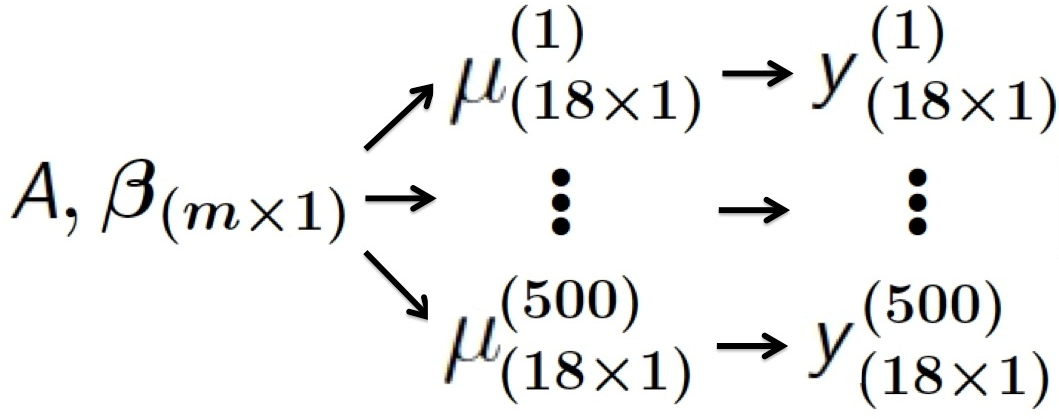
\includegraphics[width=5cm]{process.png}
\caption{Pseudo-data generating process.}
\label{fig:pseudo}
\end{center}
\end{figure}



\subsection{Coverage probability estimation}
After fitting the Gaussian model on each simulated data set, we obtain interval estimates of random effects $\boldsymbol{\mu}$. Let $(\hat{\mu}^{(i)}_{j, ~\textrm{low}}, ~\hat{\mu}^{(i)}_{j, ~\textrm{upp}})$ represent the lower and upper bounds of the interval estimate of random effect $j$ based on the $i$-th simulation given a specific confidence level.  Let's define a coverage indicator of random effect $j$ on the $i$-th mock data set as 
\begin{equation}\label{coverage_indicator}
I_{A, \boldsymbol{\beta}}(\mu_j^{(i)}) = \left\{ \begin{array}{ll}
1, & \textrm{if $\mu_j^{(i)}\in(\hat{\mu}^{(i)}_{j, ~\textrm{low}}, ~\hat{\mu}^{(i)}_{j, ~\textrm{upp}})$}\\
0, & \textrm{otherwise}
\end{array} \right.
\end{equation}
Note that an outcome of the coverage indicator depends on the simulated random effects and mock data generated by $A$ and $\boldsymbol{\beta}$. 

%Let's suppress the subscript $(r, \boldsymbol{\beta})$ from the coverage indicator for simplicity.


%B$^3$LM model to $N_{\textrm{sim}}$ pseudo-datasets in order to obtain $k\times N_{\textrm{sim}}$ interval estimates,  \{$(\hat{p}^{(i)}_{j, ~low}, ~\hat{p}^{(i)}_{j, ~upp}), ~j=1,\ldots, k,~ i=1, \ldots, N_{\textrm{sim}}$\}.  

%The simple and Rao-Blackwellized unbiased coverage estimators and their unbiased variance estimators for the coverage evaluation.  

\subsubsection{Simple unbiased coverage estimator.}
When the confidence level is 95\%, the proportion of 95\% interval estimates that contain random effect $j$ is an intuitive choice for  the coverage rate estimator for random effect $j$. This estimator  implicitly assumes that there exist $k$ unknown coverage probabilities of random effects, denoted by $C_{A, \boldsymbol{\beta}}(\mu_j)$ for $j=1, 2, \ldots, k$, depending on the values of the hyper-parameters that generate random effects and mock data sets. The coverage indicators for random effect $j$ in  \eqref{coverage_indicator} is assumed to follow an independent and identically distributed  Bernoulli distribution given the unknown coverage rate $C_{A, \boldsymbol{\beta}}(\mu_j)$. The sample mean of these coverage indicators is a simple unbiased coverage estimator for $C_{A, \boldsymbol{\beta}}(\mu_j)$;  %estimates the coverage probability via the sample mean of these indicator variables for each group $j$, 
\begin{equation}
\bar{I}_{A, \boldsymbol{\beta}}(\mu_j)= \frac{1}{N_{\textrm{sim}}}\sum_{i=1}^{N_{\textrm{sim}}}I_{A, \boldsymbol{\beta}}(\mu_j^{(i)}),~ j=1, 2, \ldots, k.
\end{equation}
Note that $\bar{I}_{A, \boldsymbol{\beta}}(\mu_j)$ averages over possible values of $\mu_{j}$ and $y_{j}$ generated by specific values of $A$ and $\boldsymbol{\beta}$. For $j=1, 2, \ldots, k$, the unbiased variance estimator of $\VAR(\bar{I}_{A, \boldsymbol{\beta}}(\mu_j))$ is 
\begin{equation}\label{svar}
\widehat{\VAR}(\bar{I}_{A, \boldsymbol{\beta}}(\mu_j))=\frac{1}{N_{\textrm{sim}}(N_{\textrm{sim}}-1)}\sum_{i=1}^{N_{\textrm{sim}}}(I_{A, \boldsymbol{\beta}}(\mu_j^{(i)})-\bar{I}_{A, \boldsymbol{\beta}}(\mu_j))^{2}.
\end{equation}

\subsubsection{Rao-Blackwellized unbiased coverage estimator.}
The frequency method checking is computationally expensive in nature because it  fits a model on every mock data set. The situation deteriorates if the number of simulations or the size of data is large, or the estimation method is computationally demanding. \citet{morris1997} and \cite{tang2002fitting} used a Rao-Blackwellized (RB) unbiased coverage estimator for the unknown coverage rate of each random effect, which is more efficient than the simple unbiased coverage estimator.  For $j=1, 2, \ldots, k$,
\begin{equation}\label{RB_theory}
C_{A, \boldsymbol{\beta}}(\mu_j)=\E(\bar{I}_{A, \boldsymbol{\beta}}(\mu_j)\vert A, \boldsymbol{\beta})=E\bigg[\frac{1}{N_{\textrm{sim}}}\sum_{i=1}^{N_{\textrm{sim}}}\E(I_{A, \boldsymbol{\beta}}(\mu_j^{(i)})\vert A, \boldsymbol{\beta}, \boldsymbol{y}^{(i)})\bigg\vert A, \boldsymbol{\beta}\bigg],
\end{equation}
where the sample mean of the conditional expectations inside the outer expectation is the RB unbiased coverage estimator. To be specific,
\begin{align}\label{RB}
\bar{I}^{RB}_{A, \boldsymbol{\beta}}(\mu_j) &= \frac{1}{N_{\textrm{sim}}}\sum_{i=1}^{N_{\textrm{sim}}}\E(I_{A, \boldsymbol{\beta}}(\mu_j^{(i)})\vert A, \boldsymbol{\beta}, \boldsymbol{y}^{(i)})\\
&= \frac{1}{N_{\textrm{sim}}}\sum_{i=1}^{N_{\textrm{sim}}} \Prob(\mu_j^{(i)}\in(\hat{\mu}^{(i)}_{j, ~\textrm{low}}, ~\hat{\mu}^{(i)}_{j, ~upp})\vert A, \boldsymbol{\beta},  \boldsymbol{y}^{(i)}).
\end{align}
We  can easily compute the above conditional posterior probabilities using the cumulative density function of the Normal conditional posterior distribution of each random effect in  \eqref{normalpost}. The variance of  $\bar{I}^{RB}_{A, \boldsymbol{\beta}}(\mu_j)$ does not exceed the variance of a simple unbiased coverage estimator $\bar{I}_{A, \boldsymbol{\beta}}(\mu_j)$ \citep{radhakrishna1945information, blackwell1947conditional}.




%, i.e., $Pr(p_j^{(i)}<\hat{p}^{(i)}_{j, ~upp}\vert r, \boldsymbol{\beta}, \boldsymbol{y}^{(i)})-Pr(p_j^{(i)}<\hat{p}^{(i)}_{j, ~low},\vert r, \boldsymbol{\beta}, \boldsymbol{y}^{(i)})$.


If one dataset $\boldsymbol{y}^{(i)}$ is simulated per one set of random effects $\boldsymbol{\mu}^{(i)}$, the variance estimator below is an unbiased estimator of $\VAR(\bar{I}^{RB}_{A, \boldsymbol{\beta}}(\mu_j) )$. For $j=1, 2, \ldots, k,$
\begin{equation}\label{RBvar}
\widehat{\VAR}(\bar{I}^{RB}_{A, \boldsymbol{\beta}}(\mu_j) )\equiv\frac{1}{N_{\textrm{sim}}(N_{\textrm{sim}}-1)}\sum_{i=1}^{N_{\textrm{sim}}}\bigg(\E(I_{A, \boldsymbol{\beta}}(\mu_j^{(i)})\vert A, \boldsymbol{\beta}, \boldsymbol{y}^{(i)})-\bar{I}^{RB}_{A, \boldsymbol{\beta}}(\mu_j) \bigg)^{2}.
\end{equation}


\subsubsection{Rao-Blackwellized overall unbiased coverage estimator}\label{overallRB} Assuming that the unknown  coverage probabilities are the same for all random effects, we use the Rao-Blackwellized overall unbiased coverage estimator and its variance estimator;
\begin{equation}\label{RBoverall}
\bar{\bar{I}}^{RB}_{r, \boldsymbol{\beta}} = \frac{1}{k}\sum_{j=1}^k\bar{I}^{RB}_{r, \boldsymbol{\beta}}(p_j)~~\textrm{and}~~ \widehat{\VAR}(\bar{\bar{I}}_{RB})=\frac{1}{k^2}\sum_{j=1}^k\widehat{\VAR}(\bar{I}^{RB}_{r, \boldsymbol{\beta}}(p_j)).
\end{equation}


\section[packageoverview]{Usage of functions in \pkg{Rgbp}}\label{sec5}
In this section, we describe the usage of the two main functions of \pkg{Rgbp}, i.e., \code{gbp} for model fitting and \code{coverage} for frequency method checking. 

\subsection{Model fitting}
The function \code{gbp} creates an S3 object ``gbp'' on which  three generic functions \code{plot}, \code{print}, and \code{summary} are defined. %To use these relevant functions, we need to save the outcome of \code{gbp} into an object such as \code{g.output} in the code below).

There are two cases according to whether covariates are available or not. When no covariates are available, the function \code{gbp} requires fitting an intercept term  or knowing the value of the  the expected random effect, meaning that the intercept term must be either estimated or known. The default of \code{gbp} in this case is to fit an intercept term. We can assign the value of the known expected random effect through an optional argument \code{mean.PriorDist}. Note that \code{gbp} can fit the Poisson model only when the value of expected random effect, $\lambda^E$, is known. The usage of \code{gbp} to  fit each model without any covariates is 
\begin{CodeChunk}
\begin{CodeInput}
R> g.output <- gbp(y, se.or.n, model = "gaussian")
R> b.output <- gbp(y, se.or.n, model = "binomial")
R> p.output <- gbp(y, se.or.n, mean.PriorDist, model = "poisson")
\end{CodeInput}
\end{CodeChunk}

The argument \code{y} is a vector of $k$ observed sample means  for the Gaussian model, $k$ observed numbers of successful outcomes for the Binomial model, and $k$ observed numbers of events happening for the Poisson model. The argument  \code{se.or.n} is a vector of $k$ standard errors of each sample mean for the Gaussian model, $k$ numbers of trials for the Binomial model, and $k$ exposures for the Poisson model. If we want to designate a known value of the expected random effect $\mu^E=\beta_1$ for the Gaussian model or $p^E=\exp(\beta_1)/(1+\exp(\beta_1))$ for the Binomial model, then we put that value into \code{gbp} using an argument \code{mean.PriorDist}. For example, if  $\mu^E$ is known as 10, then we use the following code. %The usage of the Binomial model is the same.
\begin{CodeChunk}
\begin{CodeInput}
R> g.output <- gbp(y, se.or.n, mean.PriorDist = 10, model = "gaussian")
\end{CodeInput}
\end{CodeChunk}

If covariate information for each group is available, we can fit the Gaussian and Binomial models, using the following codes.
\begin{CodeChunk}
\begin{CodeInput}
R> g.output <- gbp(y, se.or.n, X, model = "gaussian")
R> b.output <- gbp(y, se.or.n, X, model = "binomial")
\end{CodeInput}
\end{CodeChunk}

The argument \code{X} is a matrix of covariate(s) each column of which corresponds to one covariate for $k$ groups. For example, if we have two covariates for each group, the argument \code{X} must be $k\times2$ matrix to estimate three regression coefficients $\boldsymbol{\beta}=(\beta_1, \beta_2, \beta_3)$ including an intercept term, $\beta_1$, as a default. If we do not want to include an intercept term ($\beta_1=0$), estimating two regression coefficients for the two covariates, we add an optional argument \code{intercept} as follows.
\begin{CodeChunk}
\begin{CodeInput}
R> g.output <- gbp(y, se.or.n, X, model = "gaussian", intercept = FALSE)
\end{CodeInput}
\end{CodeChunk}

The function \code{gbp} contains several optional arguments. The argument \code{Alpha}, whose default value is 0.95, sets the confidence level, producing $100\times$\code{Alpha}\% interval estimates for the random effects. For the Gaussian model, setting the argument \code{normal.CI} to \code{TRUE} lets \code{gbp}  use a Normal approximation to the unconditional posterior distribution of the random effect \citep{tang2011}. The default value of \code{normal.CI} is \code{FALSE} for the skewed-Normal approximation \citep{kelly2014advances}. 

The function \code{gbp} uses the A-R method to fit the Binomial model if we assign the desired number of posterior samples ($N$ in  \eqref{weight}) through the argument \code{n.AR}; its default value is 0. There are several arguments related to the A-R method. The argument \code{n.AR.factor} determines how many trial samples the method draws; its default value is 4, meaning that the method draws \code{n.AR} $\times4$ trial samples and accepts or rejects them. The argument \code{trial.scale} is $\psi$ determining the scale parameter of the skewed-$t$ distribution (the envelope function); its default value is 1.3. The argument \code{save.result} indicates whether we save the whole posterior samples of the random effects and hyper-parameters; its default value is \code{TRUE}. The two arguments \code{t} and \code{u}, taking on positive values, allow users to choose the joint hyper-prior distribution $f(r, \boldsymbol{\beta})\propto d\boldsymbol{\beta}dr/(t+r)^{u+1}$; the default values for \code{t} and \code{u} are 0 and 1, respectively, for the joint hyper-prior distribution specified in  \eqref{eq:hyper}. 

For example, when there are two covariates, the following code produces 2,000 posterior samples of random effects and hyper-parameters, $r$ and $\boldsymbol{\beta}_{(3\times1)}$ including an intercept term, via the A-R method with 8,000 trial samples.
\begin{CodeChunk}
\begin{CodeInput}
R> b.output <- gbp(y, se.or.n, X, model = "binomial", n.AR = 2000)
\end{CodeInput}
\end{CodeChunk}

The object \code{b.output} above contains 8,000 weights (\code{b.output$weight}), 2,000 posterior samples of $\alpha$ (\code{b.output$alpha}), a $2,000\times3$ matrix of $\beta$ (\code{b.output$beta})  each column of which corresponds to 2,000 posterior samples of each regression coefficient, and a $k\times2,000$ matrix of random effects (\code{b.output$p}) each row of which has posterior samples of each random effect.


%The function \code{names} shows the list of outcomes (too many to be listed here); see the document of \code{gbp} to check the detailed list of outcomes.
%\begin{CodeChunk}
%\begin{CodeInput}
%R> names(b.output)
%R> ?gbp
%\end{CodeInput}
%\end{CodeChunk}

The S3 object ``gbp'' benefits from three generic functions, \code{print}, \code{summary}, and \code{plot}. The estimation result for all the random effects appears if we type the ``gbp'' object at the \proglang{R} console, which plays the same role of the function \code{print} with its default argument ``\code{sort = TRUE}''. When the argument \code{sort} is set to \code{TRUE}, the function \code{print} prints out the estimation result for all the groups in the ascending order of $n$ for the Binomial and Poisson model and the descending order of standard errors for the Gaussian model. When the argument \code{sort} is \code{FALSE}, the estimation result comes out in the order of data input.
\begin{CodeChunk}
\begin{CodeInput}
R> b.output
R> print(b.output, sort = FALSE)
\end{CodeInput}
\end{CodeChunk}

The function \code{summary} prints a detailed estimation result, including the estimation result for the hyper-parameters, $A$ (or $r$) and $\boldsymbol{\beta}$.
\begin{CodeChunk}
\begin{CodeInput}
R> summary(b.output)
\end{CodeInput}
\end{CodeChunk}

The function \code{plot} draws a shrinkage plot and $100\times$\code{Alpha}\% interval plot for random effects with its default argument ``\code{sort = TRUE}'' that draws the $100\times$\code{Alpha}\% interval plot in the ascending order of $n$ for the Binomial and Poisson model and the descending order of standard errors for the Gaussian model. When the argument \code{sort} is set to \code{FALSE}  the $100\times$\code{Alpha}\% interval plot is displayed in the order of data input.
\begin{CodeChunk}
\begin{CodeInput}
R> plot(b.output)
R> plot(b.output, sort = FALSE)
\end{CodeInput}
\end{CodeChunk}

\subsection{Frequency method checking}
The function \code{coverage} conducts a frequency method checking that estimates the coverage probabilities of  random effects, conditioning on the values of the hyper-parameters that generate random effects and  mock data sets. The basic usage of \code{coverage} needs a ``gbp'' object, such as \code{b.output} above, as the first argument;
\begin{CodeChunk}
\begin{CodeInput}
R> cov <- coverage(b.output, nsim = 1000)
\end{CodeInput}
\end{CodeChunk}

The argument \code{nsim} sets the number of simulations, $N_{\textrm{sim}}$, defined in Section \ref{data_generation}. If we do not assign values of the hyper-parameters through the arguments \code{A.or.r} and \code{reg.coef}, then the function \code{coverage} automatically sets the estimated posterior modes of hyper-parameters saved in the ``gbp'' object (or their posterior medians if the acceptance-rejection method for the Binomial model is used) as the generative values of hyper-parameters. If we want to conduct the frequency method checking with different generated values of hyper-parameters, for example, $r=100$ and $\boldsymbol{\beta}=(2, 5)^\top$ when one covariate was used with an intercept term, then we specify them via the arguments \code{A.or.r} and \code{reg.coef};
\begin{CodeChunk}
\begin{CodeInput}
R> cov <- coverage(b.output, A.or.r = 100, reg.coef = c(2, 5), nsim = 1000)
\end{CodeInput}
\end{CodeChunk}

When we fit a model with a known value of the expected random effect, \code{coverage} conducts the frequency method checking based on the known value. However, we may sometimes want to conduct the frequency method checking with a different value for the expected random effect. For example, if we want to try a different value of the expected random effect, e.g., 30, we add the argument \code{mean.PriorDist} as follows.
\begin{CodeChunk}
\begin{CodeInput}
R> cov <- coverage(p.output, mean.PriorDist = 30, nsim = 1000)
\end{CodeInput}
\end{CodeChunk}
The resulting frequency method checking is based on the estimated posterior mode of $r$ and the newly specified value of the expected random effect, 30.

Although the function \code{coverage} does not produce an S3 object, a detailed summary appears in a plot that automatically pops up. In addition, the variable \code{cov}  where we save  the result of \code{coverage} as above contains numerical details; $k$ RB coverage estimates (\code{cov$coverageRB}) and their standard errors (\code{cov$se.coverageRB}), $k$ simple coverage estimates (\code{cov$coverageS}) and their standard errors (\code{cov$se.coverageS}), etc.


If we save the result into an object such as \code{cov} above, then we can always recall the coverage plot, using the function \code{coverage.plot}.
\begin{CodeChunk}
\begin{CodeInput}
R> coverage.plot(cov)
\end{CodeInput}
\end{CodeChunk}


%  So, in order to generate pseudo-datasets, \code{coverage} needs parameters of prior distribution,  
%  (\emph{A} (or \emph{r}) and \eqn{\beta} (\code{reg.coef})) 
%  or (\emph{A} (or \emph{r}) and \eqn{\mu_{0}}{\mu0}). From here, we have four options to run \code{coverage}.

%  First, if any values related to the prior distribution are not designated like 
%  \code{coverage(b, nsim = 10)}, then \code{coverage} will regard estimated values (or known prior mean, \eqn{\mu_{0}}{\mu0}) in \code{b} (\code{gbp.object}) as given true values when it generates lots of pseudo-datasets. After sampling \eqn{\theta_{(i)}}{\theta_(i)} from the prior distribution determined by these estimated values (or known prior mean) in \code{b} (\code{gbp.object}), \code{coverage} creates an \emph{i}-th pseudo-dataset based on \eqn{\theta_{(i)}}{\theta_(i)} just sampled.

%  Second, \code{coverage} allows us to try different true values in generating datasets. Suppose \code{gbp.object} is based on the model with a known prior mean, \eqn{\mu_{0}}{\mu0}. Then, we can try either different \code{A.or.r} or \code{mean.PriorDist}. For example, \code{coverage(b, A.or.r = 20, nsim = 10)}, 
%\code{coverage(b, mean.PriorDist = 0.5, nsim = 10)}, or 
%\code{coverage(b, A.or.r = 20, mean.PriorDist = 0.5, nsim = 10)}. Note that we cannot set \code{reg.coef} because the second-level mean (prior mean) is known in \code{gbp.object} to begin with.

%  Suppose \code{gbp.object} is based on the model with an unknown prior mean. In this case, \code{gbp.object} has the estimation result of regression model, linear regression for Normal-Normal, log-linear regression for Poisson-Gamma, or logistic regression for Binomial-Beta, (only intercept term if there is no covariate) to estimate the unknown prior mean. Then, we can try some options: one or two of (\code{A.or.r}, \code{mean.PriorDist}, \code{reg.coef}). For example, \code{coverage(b, A.or.r = 20, nsim = 10)}, \code{coverage(b, mean.PriorDist = 0.5, nsim = 10)}, or \code{coverage(b, reg.coef = 0.1, nsim = 10)} with no covariate where \code{reg.coef} is a designated intercept term. Estimates in \code{gbp.object} will be used for undesignated values. Also, we can try appropriate combinations of two arguments. For example, \code{coverage(b, A.or.r = 20, mean.PriorDist = 0.5, nsim = 10)} and 
%\code{coverage(b, A.or.r = 20, reg.coef = 0.1, nsim = 10)}. If we have one covariate, a 2 by 1 vector should be designated for \code{reg.coef}, one for an intercept term and the other for a regression coefficient of the covariate. Note that the two arguments, \code{mean.PriorDist} and \code{reg.coef}, cannot be assigned together because we do not need \code{reg.coef} given \code{mean.PriorDist}. 

%  The simple unbiased estimator of coverage probability in \emph{j}-th group is a sample mean of indicators over all simulated datasets. The \emph{j}-th indicator in \emph{i}-th simulation is 1 if the estimated interval of the \emph{j}-th group on \emph{i}-th simulated dataset contains a true parameter 
%  \eqn{\theta_{(i)j}}{\theta_(i)j} that generated the observed value of the \emph{j}-th group in the 
%  \emph{i}-th dataset.

%  Rao-Blackwellized unbiased estimator for group \emph{j} is a conditional expectation of the simple unbiased estimator given a sufficient statistic, \eqn{y_{j}}{y_j} for Gaussian or \eqn{z_{j}}{z_j} for Binomial and Poisson data.

\section[Examples]{Examples}\label{sec6}
\subsection[Known Second-level Mean]{Data of 31 hospitals with a known expected random effect}
\label{sec:ex:hosp}


We analyze a data set of 31 hospitals in New York state comprising of the outcomes of the coronary artery bypass graft (CABG) surgery \citep{morris2012}. The data set contains the number of deaths, $\boldsymbol{y}$, for a specified period after CABG surgeries out of the total number of patients, $\boldsymbol{n}$, receiving CABG surgeries in each hospital. Health care providers may use these data to improve their care qualities, and patients may refer to the data to select a better hospital. Our goal is to obtain the point and interval estimates for the unknown true mortality rates (random effects) of 31 hospitals to evaluate  each hospital's reliability on the CABG surgery (\cite{morris1995} use a similar Poisson model to handle these hospital profile data). We interpret the caseloads, $\boldsymbol{n}$,  as exposures and assume that the state-level death rate per exposure of this surgery ($\lambda^E$) is known as 0.03 to fit the Poisson model for an illustrative purpose.  If covariate information is available or the information about the expected random effect is unknown, we recommend using the Binomial model.
%\footnote{Visit \emph{http://www.health.ny.gov/statistics/diseases/cardiovascular/} for more profile data of the CABG surgery in New York state.}

These data can be loaded into \proglang{R} using the following code.
\begin{CodeChunk}
\begin{CodeInput}
R> library("Rgbp")
R> data("hospital")
R> y <- hospital$d
R> n <- hospital$n
\end{CodeInput}
\end{CodeChunk}


%In addition, suppose one knows that the state-level death rate per exposure of this surgery is 0.030 ($\lambda_{0}$). Using these data and the known second-level mean ($\lambda_{0}$), \pkg{Rgbp} provides point and interval estimates of the true death rate ($\lambda_{j}$) so that one can evaluate each hospital's reliability. 


%The independent Poisson distribution, i.e.,  $y_j\vert \lambda_j\stackrel{indep.}{\sim} \textrm{Poisson}(n_{j}\lambda_{j})$, $j=1, \ldots, 31,$ would be an ideal choice to describe these data based on the Poisson approximation when $\lambda$ is small and $n$ is relatively large. 


The function \code{gbp} fits the Poisson model with a Gamma conjugate prior distribution as the population distribution of the death rates in New York states whose mean ($\lambda^E$) is 0.030. The number of regression coefficients ($m$) is 0 because we do not estimate them via  a log-linear regression. 
\begin{CodeChunk}
\begin{CodeInput}
R> p.output <- gbp(z, n, mean.PriorDist = 0.03, model = "poisson")
R> p.output
\end{CodeInput}
\begin{CodeOutput}
Summary for each unit (sorted by n):

      obs.mean    n prior.mean shrinkage low.intv post.mean upp.intv post.sd
1       0.0448   67       0.03     0.911   0.0199    0.0313   0.0454 0.00653
2       0.0294   68       0.03     0.910   0.0189    0.0299   0.0435 0.00631
3       0.0238  210       0.03     0.765   0.0185    0.0285   0.0407 0.00566
4       0.0430  256       0.03     0.728   0.0225    0.0335   0.0467 0.00619
5       0.0335  269       0.03     0.718   0.0208    0.0310   0.0432 0.00573
6       0.0438  274       0.03     0.714   0.0229    0.0339   0.0472 0.00621
7       0.0432  278       0.03     0.711   0.0228    0.0338   0.0469 0.00617
8       0.0136  295       0.03     0.699   0.0157    0.0250   0.0366 0.00534
9       0.0288  347       0.03     0.663   0.0200    0.0296   0.0410 0.00536
10      0.0372  349       0.03     0.662   0.0222    0.0325   0.0446 0.00571
11      0.0391  358       0.03     0.656   0.0228    0.0331   0.0454 0.00579
12      0.0177  396       0.03     0.633   0.0165    0.0255   0.0363 0.00506
13      0.0278  431       0.03     0.613   0.0200    0.0292   0.0400 0.00511
14      0.0249  441       0.03     0.608   0.0191    0.0280   0.0387 0.00502
15      0.0273  477       0.03     0.589   0.0199    0.0289   0.0394 0.00499
16      0.0455  484       0.03     0.585   0.0256    0.0364   0.0491 0.00601
17      0.0304  494       0.03     0.580   0.0211    0.0302   0.0409 0.00506
18      0.0220  501       0.03     0.577   0.0180    0.0266   0.0369 0.00483
19      0.0277  505       0.03     0.575   0.0202    0.0290   0.0395 0.00494
20      0.0204  540       0.03     0.559   0.0173    0.0258   0.0358 0.00474
21      0.0284  563       0.03     0.548   0.0206    0.0293   0.0395 0.00485
22      0.0236  593       0.03     0.535   0.0187    0.0270   0.0369 0.00466
23      0.0150  602       0.03     0.532   0.0147    0.0230   0.0329 0.00466
24      0.0238  629       0.03     0.521   0.0188    0.0271   0.0368 0.00460
25      0.0204  636       0.03     0.518   0.0173    0.0254   0.0351 0.00455
26      0.0480  729       0.03     0.484   0.0286    0.0393   0.0516 0.00587
27      0.0306  849       0.03     0.446   0.0223    0.0303   0.0397 0.00445
28      0.0274  914       0.03     0.428   0.0208    0.0285   0.0374 0.00423
29      0.0213  940       0.03     0.421   0.0176    0.0249   0.0335 0.00407
30      0.0293 1193       0.03     0.364   0.0223    0.0296   0.0379 0.00397
31      0.0201 1340       0.03     0.338   0.0170    0.0235   0.0310 0.00360
Mean            517       0.03     0.600   0.0201    0.0293   0.0403 0.00517
\end{CodeOutput}
\end{CodeChunk}

The output contains information about the observed death rates $\bar{y}_{j}$, caseloads $n_{j}$, known prior mean $\lambda^E$, shrinkage estimates $\hat{B}_{j}$, lower bounds of interval estimates $\hat{\lambda}_{j, \textrm{low}}$, posterior means $\hat{\lambda}_j$, upper bounds  of interval estimates $\hat{\lambda}_{j, \textrm{upp}}$, and posterior standard deviations  for each random effect based on the assumed unconditional Gamma posterior distributions. %The lower and upper bounds of an interval estimate for a random effect are 2.5\% and 97.5\% percentiles of the assumed unconditional Gamma posterior distributions if 95\% confidence level is used.

%Note that the conditional posterior mean of random effect $j$ in Equation \ref{gammapost_mean_var} is $(1-B_{j})\bar{y}_{j} + B_{j}\lambda^E$,  a convex combination of the observed death rate and expected random effect with the shrinkage factor, $B_{j}\equiv r / (r + n_{j})$, determining the weight. This makes intuitive sense because $r$ and $n_{j}$ can be interpreted as the degree (sample sizes) of prior and observed information respectively. If the second level has more information than the first level, i.e., ensemble sample size $r$ exceeds individual sample size $n_{j}$, then the estimator will shrink towards the prior mean more than 50\%. This is clear because, as caseload increases, shrinkage decreases, depending less on the  state-level (second-level) conjugate Gamma prior distribution.


A function \code{summary} shows selective information about hospitals with minimum, median, and maximum exposures and the estimation result of the hyper-parameter $\alpha=-\log(r)$.  \begin{CodeChunk}
\begin{CodeInput}
R> summary(p.output)
\end{CodeInput}
\begin{CodeOutput}
Main summary:

                    obs.mean    n prior.mean shrinkage low.intv post.mean
Unit with min(n)      0.0448   67       0.03     0.911   0.0199    0.0313   
Unit with median(n)   0.0455  484       0.03     0.585   0.0256    0.0364   
Unit with max(n)      0.0201 1340       0.03     0.338   0.0170    0.0235   
Overall Mean                  517       0.03     0.600   0.0201    0.0293   

                    upp.intv  post.sd
                      0.0454  0.00653
                      0.0491  0.00601
                      0.0310  0.00360
                      0.0403  0.00517

Second-level Variance Component Estimation Summary:
alpha=log(A) for Gaussian or alpha=log(1/r) for Binomial and Poisson data:

post.mode.alpha post.sd.alpha post.mode.r
          -6.53         0.576         684
\end{CodeOutput}
\end{CodeChunk}
The output of \code{summary} shows that $\hat{r}=\textrm{exp}(6.53)=684$, which is an indicator of how valuable and informative the second-level hierarchy is. It means that observed sample means of hospitals whose caseloads are less than 684 shrink toward the prior mean (0.030) more than 50\%. For example, the shrinkage estimate of the first hospital ($\hat{B}_{1}= 0.911$) was calculated by 684 / (684 + 67), where 67 is its caseload ($n_{1}$), and its posterior mean is $(1-0.911)*0.0448 + 0.911 * 0.030=0.0313$. As for this hospital, using more information from the conjugate prior distribution is an appropriate choice because the amount  of observed information (67) is much less than the amount of state-level information (684).


To obtain a graphical summary, we use the function \code{plot}.%, as seen in Figure \ref{fig:hospshr}.

\begin{CodeChunk}
\begin{CodeInput}
R> plot(p.output)
\end{CodeInput}
\end{CodeChunk}
\begin{figure}[h]
\begin{center}
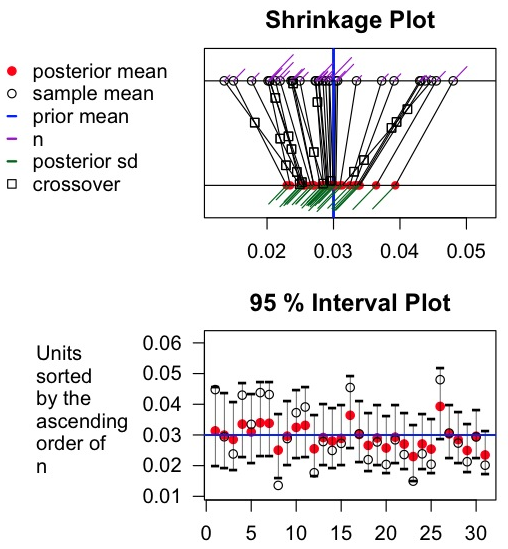
\includegraphics[width = 2.8in]{hospital1.png}
\caption{Shrinkage plot and 95\% interval plot for 31 hospitals.}
\label{fig:hospshr}
\end{center}
\end{figure}

In Figure \ref{fig:hospshr} the regression towards the mean (RTTM) is obvious in the first plot; the observed death rates, denoted by empty dots on the upper horizontal line, are shrinking towards the known expected random effect, denoted by a blue vertical line at 0.03, to the different extents. Note that some hospitals' ranks have changed by shrinking much harder towards 0.03 than the others. For example, an empty square at the crossing point of the two left-most lines (8th and 23rd hospitals on the list above) indicates that  the seemingly safest hospital in terms of the observed death rate is probably not the safest in terms of the estimated posterior mean accounting for the different caseloads of these two hospitals. 

%Intuitively, switching ranks for these two hospitals is reasonable. 
To be specific, their observed death rates ($y_{j}$, $j=8, 23$) are 0.0136 and 0.0150 and caseloads ($n_{j}$, $j=8, 23$) are 295 and 602, respectively. Considering solely the observed death rates may lead to an unfair comparison because the latter hospital handled twice the caseload. \pkg{Rgbp} accounts for this caseload difference, making the posterior mean for the random effect of the former hospital shrink toward the state-level mean ($\lambda^E$=0.03) much harder than that for the latter hospital.


Note that the point estimates are not enough to evaluate hospital reliability because one hospital may have a lower point estimate but  larger uncertainty (variance) than the other. The second plot of Figure \ref{fig:hospshr} displays the 95\% interval estimates. Note that each posterior mean (red dot) is between the sample mean (empty dot) and the known expected random effect (a blue horizontal line). %For reference, we could plot this 95\% interval plot by the order of data input via \code{plot(p, sort = FALSE)}.

This 95\% interval plot reveals that the 31st hospital has the lowest upper bound even though its point estimate ($\hat{\lambda}_{31}=0.0235$) is slightly larger than that of the 23rd hospital ($\hat{\lambda}_{23}=0.0230$). The observed death rates for these two hospitals ($y_{j}, j=23, 31$) are 0.0150 and 0.0201 and the caseloads ($n_{j}, j =23, 31$) are 602 and 1340 each. The 31st hospital has twice the caseload, which leads to borrowing less information from the New York state-level hierarchy (or shrinking less toward the state-level mean, 0.03) with smaller variance. Based on the point and interval estimates, the 31st hospital seems the most reliable one.

We conduct the frequency method checking to question how reliable the estimation procedure is.  The function \code{coverage}  generates pseudo-datasets given the estimated value of $r$, 683.53, as a generative value. For reference, we can designate any generative values of $r$ and $\lambda^E$ by adding two arguments, \code{A.or.r} and \code{mean.PriorDist}, into the code below.
%; \code{R> pcv <- coverage(p, A.or.r = 600, nsim = 1000)}.
%For example, does our procedure generate interval estimates that have good repeated sampling properties? To answer this question 

%In addition, \code{gbp} also provides interval estimates with different confidence levels, for example 90\%. For this, we need to go back to the code for fitting the model, adding another argument, \code{Alpha = 0.9}; \code{R> p <- gbp(z, n, Alpha = 0.9, mean.PriorDist = 0.03, model = "poisson")}.  Then, the code below will evaluate whether interval estimates achieve the 90\% confidence level.

\begin{CodeChunk}
\begin{CodeInput}
R> p.coverage <- coverage(p.output, nsim = 1000)
\end{CodeInput}
\end{CodeChunk}
\begin{figure}[h] 
\begin{center}
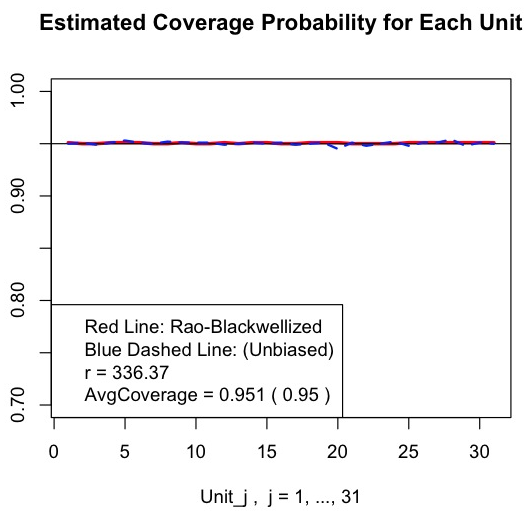
\includegraphics[width = 2.8in]{hospital2.png}
\caption{Coverage plot via frequency method checking for 31 hospitals.}
\label{fig:hospitalcoverage}
\end{center}
\end{figure}

In Figure \ref{fig:hospitalcoverage}, the black horizontal line at 0.95 represents the nominal confidence level  and the red circles indicate RB unbiased coverage estimates, $\bar{I}^{RB}_{r, \lambda^\E}(\lambda_j)$ for $j=1, 2, \ldots, 31$. The overall RB unbiased coverage estimate across all the hospitals ($\bar{\bar{I}}^{RB}_{r, \lambda^E}$) is 0.955. None of RB unbiased coverage estimates for 31 hospitals are less than 0.95 regardless of their caseloads. This result shows that the interval estimates for this particular dataset accurately achieves 95\% confidence level. 

%Note that these estimates depend on the given true value of $r$ the known prior mean, and the assumption that the model is true.

The following code provides specific values of the 31 RB unbiased coverage estimates and their standard errors for each hospital (the output is omitted for a space concern).
\begin{CodeChunk}
\begin{CodeInput}
R> p.coverage$coverageRB
R> p.coverage$se.coverageRB
\end{CodeInput}
%\begin{CodeOutput}
% [1] 0.955 0.954 0.955 0.954 0.954 0.954 0.954 0.954 0.954 0.954 0.954 0.954
%[13] 0.954 0.953 0.953 0.954 0.953 0.954 0.954 0.953 0.953 0.953 0.954 0.953
%[25] 0.953 0.953 0.952 0.953 0.952 0.952 0.952
%\end{CodeOutput}
\end{CodeChunk}

And the code below shows 31 simple unbiased coverage estimates and their standard errors for each hospital.
\begin{CodeChunk}
\begin{CodeInput}
R> p.coverage$coverageS
R> p.coverage$se.coverageS
\end{CodeInput}
%\begin{CodeOutput}
% [1] 0.949 0.960 0.958 0.958 0.950 0.945 0.960 0.953 0.960 0.956 0.955 0.946 
%[13] 0.955 0.954 0.960 0.965 0.955 0.952 0.960 0.956 0.959 0.955 0.964 0.960 
%[25] 0.945 0.942 0.947 0.960 0.940 0.946 0.956
%\end{CodeOutput}
\end{CodeChunk}

%The function \code{coverage} also calculates the standard errors for each hospital's RB unbiased coverage estimate defined in (\ref{RBvar}). The following code provides 31 standard errors for RB estimates.
%\begin{CodeChunk}
%\begin{CodeInput}
%\end{CodeInput}
%\begin{CodeOutput}
% [1] 0.0016 0.0016 0.0014 0.0014 0.0013 0.0013 0.0013 0.0013 0.0012 0.0013 0.0012 
%[12] 0.0012 0.0011 0.0011 0.00110.0011 0.0011 0.0011 0.0011 0.0011 0.0010 0.0010 
%[23] 0.0010 0.0010 0.0010 0.0009 0.0009 0.0008 0.0008 0.0007 0.0007
%\end{CodeOutput}
%\end{CodeChunk}
%Similarly, 31 standard errors for each simple unbiased coverage estimate defined in (\ref{svar}) are
%\begin{CodeChunk}
%\begin{CodeInput}

%\end{CodeInput}
%\begin{CodeOutput}
% [1] 0.0070 0.0062 0.0063 0.0063 0.0069 0.0072 0.0062 0.0067 0.0062 0.0065 0.0066
%[12] 0.0072 0.0066 0.0066 0.0062 0.0058 0.0066 0.0068 0.0062 0.0065 0.0063 0.0066 
%[23] 0.0059 0.0062 0.0072 0.0074 0.0071 0.0062 0.0075 0.0072 0.0065
%\end{CodeOutput}
%\end{CodeChunk}

It turns out that the variance estimate of the RB unbiased coverage estimate for the first hospital ($0.0016^2$) is about 19 times smaller than that of the simple one ($0.0070^2$). It means that the RB unbiased coverage estimates based on 1,000 simulations ($N_{\textrm{sim}}$) are as precise as the simple unbiased coverage estimates based on 19,000 simulations in terms of estimating the coverage probability for the first hospital, $C_{r, \lambda^\E}(\lambda_1)$.

%For reference, two $31 \times 1,000$ matrices \code{raw.resultRB} and \code{raw.resultS}, each row of which is about each hospital, in \code{pcv} contain all the individual estimates, $I^{(i)}_{j}$ and $E(I^{(i)}_{j}\vert y^{(i)}_{j}, A, \boldsymbol{\beta})$.

%See \cite{1995} for a similar ranking problem using a Poisson hierarchical modeling with a different parametrization.


\subsection[Unknown Second-level Mean and No Covariate]{Data of 8 schools with unknown expected random effect and no covariates} \label{sec:ex:8schools}

The Education Testing Service (ETS) conducted randomized experiments in eight separate schools (groups) to test whether students (units) SAT scores are effected by coaching. The dataset contains the estimated coaching effects on SAT scores ($y_{j}, j=1, \ldots, 8$) and standard errors ($se_{j}, j=1, \ldots, 8$) of the eight schools \citep{1981}. We can load this data set into \proglang{R} by the following codes.
\begin{CodeChunk}
\begin{CodeInput}
R> library("Rgbp")
R> data("schools")
R> y  <- schools$y
R> se <- schools$se
\end{CodeInput}
\end{CodeChunk}



Due to the nature of the test each school's coaching effect has an approximately Normal sampling distribution with known sampling variance, i.e., standard error of each school is completely known. At the second hierarchy, the mean for each school is assumed to be drawn from a common Normal distribution and hence, we can use the Gaussian component of \code{gbp} to fit this Gaussian hierarchical model.


\begin{CodeChunk}
\begin{CodeInput}
R> g.output <- gbp(y, se, model = "gaussian")
R> g.output
\end{CodeInput}
\begin{CodeOutput}
Summary for each group (sorted by the descending order of se): 

     obs.mean   se prior.mean shrinkage low.intv post.mean upp.intv post.sd
8       12.00 18.0       8.17     0.734   -10.21      9.19     29.9   10.23
3       -3.00 16.0       8.17     0.685   -17.13      4.65     22.5   10.10
1       28.00 15.0       8.17     0.657    -2.32     14.98     38.8   10.56
4        7.00 11.0       8.17     0.507    -8.78      7.59     23.6    8.26
6        1.00 11.0       8.17     0.507   -13.03      4.63     20.1    8.44
2        8.00 10.0       8.17     0.459    -7.25      8.08     23.4    7.81
7       18.00 10.0       8.17     0.459    -1.29     13.48     30.8    8.18
5       -1.00  9.0       8.17     0.408   -13.30      2.74     16.7    7.63
Mean          12.5       8.17     0.552    -9.16      8.17     25.7    8.90
\end{CodeOutput}
\end{CodeChunk}
This output from \code{gbp} summarizes the results. In this Gaussian hierarchical model the amount of shrinkage for each unit is governed by the shrinkage factor, $B_j = V_j/(V_j + A)$. As such, schools whose variation within the school ($V_{j}$) is less than the between school variation ($A$) will shrink greater than $50\%$. The results provided by \code{gpb} suggests that there is little evidence that the training provided much added benefit due to the fact that every school's $95\%$ posterior interval contains 0. In the case where the number of groups is large \pkg{Rgbp} provides a summary feature:

\begin{CodeChunk}
\begin{CodeInput}
R> summary(g.output)
\end{CodeInput}
\begin{CodeOutput}
Main summary:

                      obs.mean   se prior.mean shrinkage low.intv post.mean
Unit with min(se)        -1.00  9.0       8.17     0.408   -13.30      2.74     
Unit with median(se)1     1.00 11.0       8.17     0.507   -13.03      4.63     
Unit with median(se)2     7.00 11.0       8.17     0.507    -8.78      7.59     
Unit with max(se)        12.00 18.0       8.17     0.734   -10.21      9.19     
Overall Mean                   12.5       8.17     0.552    -9.16      8.17     

                      upp.intv post.sd
                          16.7    7.63
                          20.1    8.44
                          23.6    8.26
                          29.9   10.23
                          25.7    8.90

Second-level Variance Component Estimation Summary:
alpha=log(A) for Gaussian or alpha=log(1/r) for Binomial and Poisson data:

post.mode.alpha post.sd.alpha post.mode.A
           4.77          1.14         118


Regression Summary:

      estimate   se z.val p.val
beta1    8.168 5.73 1.425 0.154
\end{CodeOutput}
\end{CodeChunk}
The summary provides results regarding the second level hierarchy parameters. It can be seen that the estimate of the expected random effect, $\mu^E=\beta_1$ (\code{beta1}), is not significantly different from 0 suggesting that there was no effect of the coaching program on SAT math scores. 


\pkg{Rgbp} also provides functionality to plot the results of the analysis as seen in Figure \ref{fig:8schoolsplot}. Plotting the results provides a visual aid to understanding but is only largely beneficial when the number of groups $(k)$ is small. 

\begin{CodeChunk}
\begin{CodeInput}
R> plot(g.output)
\end{CodeInput}
\end{CodeChunk}

\begin{figure}[h] 
\begin{center}
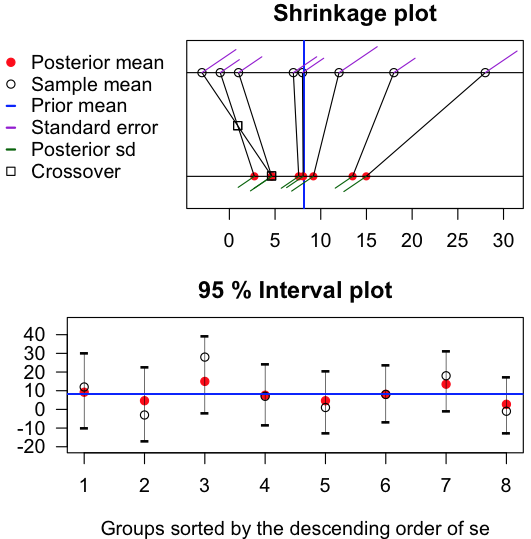
\includegraphics[width = 2.8in]{school1.png}
\caption{Shrinkage plot and 95\% interval plot for 8 schools.}
\label{fig:8schoolsplot}
\end{center}
\end{figure}


The frequency method checking generates new pseudo-data from our assumed model. Unless otherwise specified, the procedure fixes the hyper-parameter values at their estimates ($\hat{A}$ and $\hat{\boldsymbol{\beta}}_1$ in this example) and then simulates random effects $\theta_j$ for each group $j$. The model is then estimated and this is repeated an $N_{\textrm{sim}}$ (\code{nsim}) number of times to estimate the coverage probabilities of the procedure.  

\begin{CodeChunk}
\begin{CodeInput}
R> g.coverage <- coverage(g.output, nsim = 1000)
\end{CodeInput}
\end{CodeChunk}
\begin{figure}[h!] 
\begin{center}
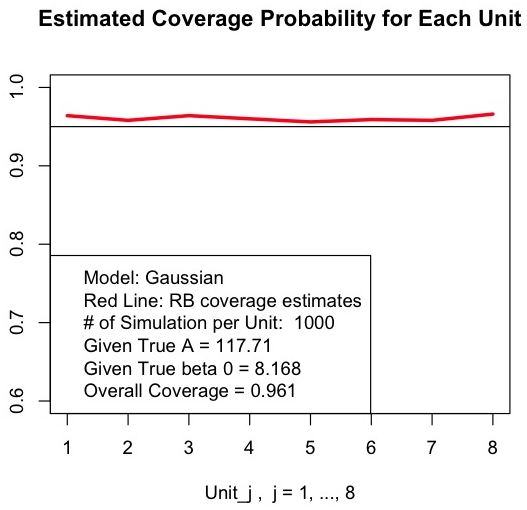
\includegraphics[width = 2.8in]{school2.png}
\caption{Coverage plot via frequency method checking for 8 schools.}
\label{fig:schoolcoverage}
\end{center}
\end{figure}

As seen in Figure \ref{fig:schoolcoverage} the desired $95\%$ confidence level, denoted by a black horizontal line at 0.95, is achieved for each school in this example. Note that all the coverage estimates depend on the chosen generative values of $A$ and $\beta_{1}$, and the assumption that the model is valid.


In addition, Rao-Blackwellized (RB) unbiased coverage estimate and its standard error for each school can be gotten with the command below.
\begin{CodeChunk}
\begin{CodeInput}
R> g.coverage$coverageRB
\end{CodeInput}
\begin{CodeOutput}
 [1] 0.966 0.959 0.967 0.960 0.959 0.962 0.960 0.966
\end{CodeOutput}
\end{CodeChunk}
\begin{CodeChunk}
\begin{CodeInput}
R> g.coverage$se.coverageRB
\end{CodeInput}
\begin{CodeOutput}
 [1] 0.0013 0.0012 0.0013 0.0013 0.0011 0.0011 0.0010 0.0017
\end{CodeOutput}
\end{CodeChunk}

All the individual RB coverage estimates are saved in the $8\times1,000$ matrix, each row of which is about each school. We can load this matrix by the following code.
\begin{CodeChunk}
\begin{CodeInput}
R> g.coverage$raw.resultRB 
\end{CodeInput}
\end{CodeChunk}




% For reference, it took 188 seconds for 10,000 simulations  on one of authors' MacBook Pro with a 2.3 GHz dual-core Intel i5 CPU. In MCMC, the exact simulation would be too time-consuming. One could compare curve in Figure \ref{fig:schoolcoverage} with a curve from MCMC.

%\begin{CodeChunk}
%\begin{CodeInput}
%R> shr <- seq(0.01, 0.99, length.out = 20)
%R> A.trial <- mean(n) * (1 - shr) / shr
%R> cov.save <- sapply (1 : length(A.trial), function(i){
%R>               coverage(g, A.or.r = A.trial[i], reg.coef = 8.168, 
%R>                        nsim = 500)$average.coverageRB
%R>             })
%\end{CodeInput}
%\end{CodeChunk}
%\begin{figure}[h]
%\begin{center}
%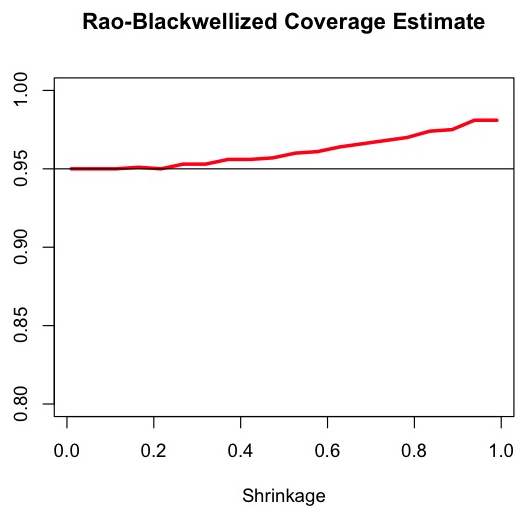
\includegraphics[width = 5.5cm]{school3.png}
%\end{center}
%\end{figure}


\subsection[Unknown Second-level Mean and One Covariate]{Data of 18 baseball players with unknown expected random effect and one covariate} 

The data of 18 major league baseball players contain the batting averages through their first 45 official at-bats of the 1970 season \citep{1975}. We add a binary covariate that takes on one if a player is an outfielder and zero otherwise. We can load the data into \proglang{R} with the following codes.
\begin{CodeChunk}
\begin{CodeInput}
R> library("Rgbp")
R> data("baseball")
R> y <- baseball$Hits
R> n <- baseball$At.Bats
R> x <- ifelse(baseball$Position == "fielder", 1, 0)
\end{CodeInput}
\end{CodeChunk}
%$
Conditioning on the unknown true batting average (random effect) of each player we assume that the at-bats are independent and therefore, $y_{j}\vert p_{j}\stackrel{\textrm{indep.}}{\sim} \textrm{Binomial}(45,~ p_{j}), ~j=1, \ldots, 18$. Our goal is to obtain point and interval estimates of each random effect whilst considering the additional information on whether the player is an outfielder or not. The function \code{gbp} provides a way to incorporate such covariate information seamlessly into the model so that the regression towards the mean (RTTM) occurs within outfielders and non-outfielders separately. %For reference, we can also assume the Normal distribution using $y_{j}=z_{j} / n_{j}$ and $V_{j}=\bar{y}(1-\bar{y})/n$, where $\bar{y}=\sum_{j} z_{j} / \sum_{j} n_{j}$, $j=1,\ldots, 18$. 


\begin{CodeChunk}
\begin{CodeInput}
R> b.output <- gbp(z, n, x, model = "binomial")
R> b.output
\end{CodeInput}
\begin{CodeOutput}
Summary for each unit (sorted by n):

     obs.mean  n  X1 prior.mean shrinkage low.intv post.mean upp.intv post.sd
1       0.400 45 1.0      0.310     0.715    0.248     0.335    0.429  0.0462
2       0.378 45 1.0      0.310     0.715    0.244     0.329    0.420  0.0448
3       0.356 45 1.0      0.310     0.715    0.240     0.323    0.411  0.0437
4       0.333 45 1.0      0.310     0.715    0.236     0.316    0.403  0.0429
5       0.311 45 1.0      0.310     0.715    0.230     0.310    0.396  0.0424
6       0.311 45 0.0      0.233     0.715    0.179     0.256    0.341  0.0415
7       0.289 45 0.0      0.233     0.715    0.175     0.249    0.331  0.0400
8       0.267 45 0.0      0.233     0.715    0.171     0.243    0.323  0.0388
9       0.244 45 0.0      0.233     0.715    0.166     0.237    0.315  0.0380
10      0.244 45 1.0      0.310     0.715    0.210     0.291    0.379  0.0432
11      0.222 45 0.0      0.233     0.715    0.161     0.230    0.308  0.0377
12      0.222 45 0.0      0.233     0.715    0.161     0.230    0.308  0.0377
13      0.222 45 0.0      0.233     0.715    0.161     0.230    0.308  0.0377
14      0.222 45 1.0      0.310     0.715    0.202     0.285    0.375  0.0441
15      0.222 45 1.0      0.310     0.715    0.202     0.285    0.375  0.0441
16      0.200 45 0.0      0.233     0.715    0.155     0.224    0.302  0.0377
17      0.178 45 0.0      0.233     0.715    0.148     0.218    0.297  0.0381
18      0.156 45 0.0      0.233     0.715    0.140     0.211    0.292  0.0389
Mean          45 0.4      0.267     0.715    0.191     0.267    0.351  0.0410
\end{CodeOutput}
\end{CodeChunk}
% Our model reflects on the additional information, \emph{i.e.}, indicator covariate (1 for outfielder and 0 for other positions), estimating two different prior means, 0.310 and 0.233. Also

Note that the shrinkage estimates are the same for all players because all players have the same 45 at-bats. %they are determined solely by the relative amount of information between the first-level and the second-level hierarchies, ($\hat{B}_{j}\equiv \hat{r} / (\hat{r}+45)$ = $113 / (113+45)$ = 0.715). 


\begin{CodeChunk}
\begin{CodeInput}
R> summary(b.output)
\end{CodeInput}
\begin{CodeOutput}
Main summary:

                            obs.mean  n    X1 prior.mean shrinkage low.intv 
Unit with min(obs.mean)        0.156 45 0.000      0.233     0.715    0.140     
Unit with median(obs.mean)1    0.244 45 0.000      0.233     0.715    0.166     
Unit with median(obs.mean)2    0.244 45 1.000      0.310     0.715    0.210     
Unit with max(obs.mean)        0.400 45 1.000      0.310     0.715    0.248     
Overall Mean                         45 0.444      0.267     0.715    0.191     


                            post.mean upp.intv post.sd
                                0.211    0.292  0.0389
                                0.237    0.315  0.0380
                                0.291    0.379  0.0432
                                0.335    0.429  0.0462
                                0.267    0.351  0.0410

Second-level Variance Component Estimation Summary:
alpha=log(A) for Gaussian or alpha=log(1/r) for Binomial and Poisson data:

post.mode.alpha post.sd.alpha post.mode.r
          -4.73         0.957         113


Regression Summary:

      estimate    se  z.val p.val
beta1   -1.194 0.131 -9.129 0.000
beta2    0.389 0.187  2.074 0.038
\end{CodeOutput}
\end{CodeChunk}

The regression coefficient for the outfielder indicator is significant, considering that $p$~value for $\hat{\beta}_2$ is 0.038. It means that the  two estimates for the expected random effects for the outfielders and infielders are significantly different. Also, the positive sign of $\hat{\beta}_{2}$ indicates that the population batting average for all outfielders tends to be higher than that for infielders. The  estimated odds ratio is $\exp(0.389)=1.48$.

\begin{CodeChunk}
\begin{CodeInput}
R> plot(b.output)
\end{CodeInput}
\end{CodeChunk}
\begin{figure}[h!]
\begin{center}
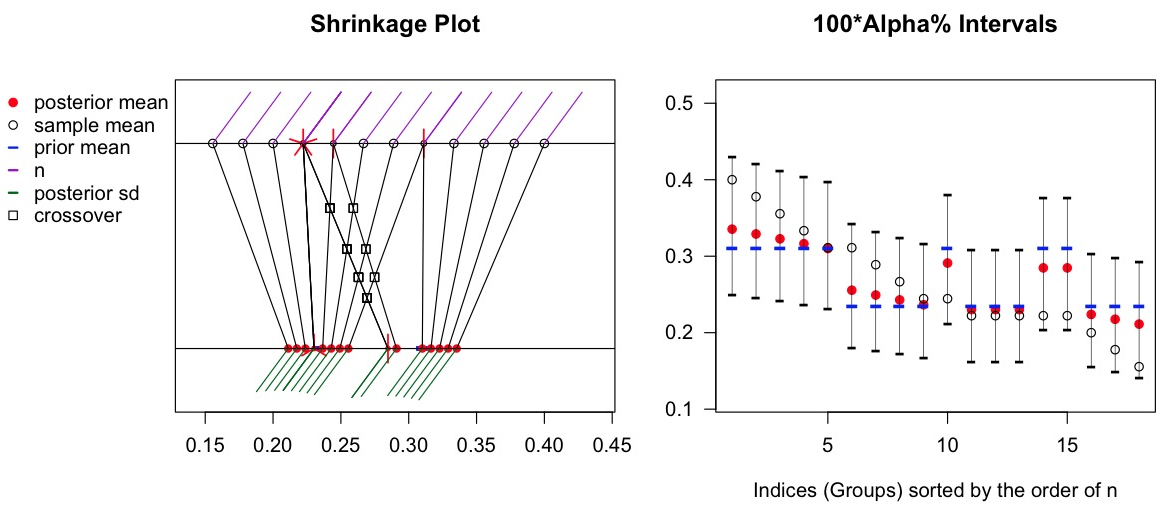
\includegraphics[width = 2.8in]{baseball1.png}
\caption{Shrinkage plot and 95\% interval plot for 18 baseball players.}
\label{fig:baseball}
\end{center}
\end{figure}

The shrinkage plot in Figure \ref{fig:baseball} shows that  the observed batting averages (empty dots) on the upper horizontal line shrink towards the two expected random effects, 0.233 and 0.310. The short red line symbols near some empty dots are for when two or more points have the same mean and are plotted over each other. For example, five players (from the 11th player to the 15th) have the same batting average, 0.222, and at this point on the upper horizontal line, there are short red lines toward five directions.

%For reference, the observed sample mean among outfielders is 0.308 and that among other positions is 0.231. But why are the estimated two prior means from this Binomial model 0.310 and 0.233 each? This can be attributed to the logistic regression which estimates prior mean by a non-linear logit function of $x'\beta$, causing a small bias (see 3.3). The Normal model can avoid this small bias because it uses a linear regression to estimate these prior means.


The 95\% interval plot in Figure \ref{fig:baseball} shows the range of true batting average for each player, which clarifies the regression toward the mean (RTTM) within two groups. The 10th, 14th, and 15th players, for example, are outfielders but their observed batting averages are far lower than the first five outfielders. This can  be attributed to their bad luck because their observed batting averages are close to the lower bounds of their interval estimates. The RTTM indicates that their batting averages  shrink towards the expected random effect of outfielders (0.310) in the long run.


To check the level of trust in these interval estimates, we  proceed to frequency method checking by assuming the estimates, 112.95 for $\hat{r}$ and (-1.194, ~0.389) for $\hat{\boldsymbol{\beta}}$, are the generative values. 

\begin{CodeChunk}
\begin{CodeInput}
R> b.coverage <- coverage(b.output, nsim = 1000) 
\end{CodeInput}
\end{CodeChunk}
\begin{figure}[h!]
\begin{center}
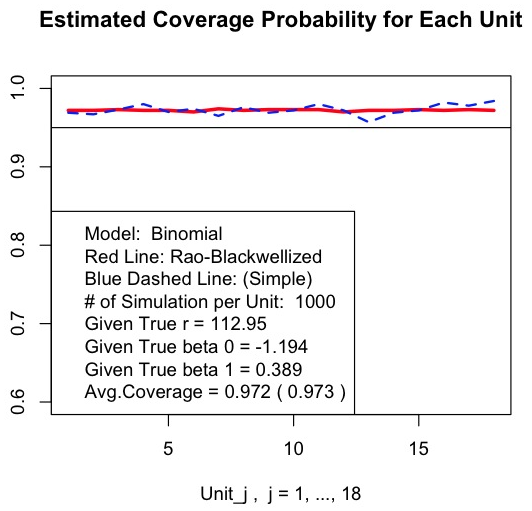
\includegraphics[width = 2.8in]{baseball2.png}
\caption{Coverage plot via frequency method checking for 18 players.}
\label{fig:baseball2}
\end{center}
\end{figure}

%For reference, to do the frequency method checking at different true values, we need to specify additional arguments in the coverage function. For example, if we want to try different true values, either 100 for $r$ or (-1, 0.2) for $(\beta_{0}, \beta_{1})$, the additional arguments are \code{A.or.r = 100} and \code{reg.coef = c(-1, 0.2)}; \code{coverage(b, A.or.r = 100, reg.coef = c(-1, 0.2), nsim = 1000)}.


In Figure \ref{fig:baseball2},  the estimated coverage probabilities for random effects are beyond 0.95, conservatively satisfying the 95\% confidence level. The RB overall unbiased coverage estimate across all the players is 0.972. Note that each coverage estimate depends on given true values of $r$ and $\boldsymbol{\beta}_{(2\times1)}$, and the assumption that the model is valid (overdispersion exists).


We can check the RB unbiased coverage estimates and their standard errors for each player.
\begin{CodeChunk}
\begin{CodeInput}
R> bcv$coverageRB
\end{CodeInput}
%$
\begin{CodeOutput}
 [1] 0.971 0.973 0.972 0.972 0.970 0.973 0.973 0.974 0.973 0.973 0.971 0.973 
[13] 0.973 0.972 0.972 0.971 0.973 0.971
\end{CodeOutput}
\end{CodeChunk}
\begin{CodeChunk}
\begin{CodeInput}
R> bcv$se.coverageRB
\end{CodeInput}
\begin{CodeOutput}
 [1] 0.0015 0.0012 0.0013 0.0014 0.0016 0.0010 0.0012 0.0010 0.0010 0.0013 
[11] 0.0015 0.0013 0.0019 0.0013 0.0014 0.0015 0.0011 0.0014
\end{CodeOutput}
\end{CodeChunk}

%$

%All the simulation results are saved in the $18\times1,000$ matrix, each row of which is for each player.

%$

If we want to draw 2,000 posterior samples of random effects and hyper-parameters from their full posterior distribution via the A-R method, we use the following \proglang{R} code.
\begin{CodeChunk}
\begin{CodeInput}
R> b.output <- gbp(y, n, x, model = "binomial", n.AR = 2000)
\end{CodeInput}
\end{CodeChunk}
The ``gbp'' object \code{b.output} contains 8,000 weights (\code{b.output$weight}), 2,000 posterior samples of $\alpha$ (\code{b.output$alpha}), a $2,000\times2$ matrix of $\beta$ (\code{b.output$beta})  each column of which corresponds to 2,000 posterior samples of each regression coefficient, and a $k\times2,000$ matrix of random effects (\code{b.output$p}) each row of which has posterior samples of each random effect.

If we run the frequency method checking using this ``gbp'' object obtained via the A-R method, the $N_{\textrm{sim}}$ simulations also run the A-R method each time.

\section[Discussion]{Discussion} \label{discussion}
\pkg{Rgbp} is an \proglang{R} package for estimating and validating two-level Gaussian, Poisson, and Binomial hierarchical models. The package aims to provide a procedure that is computationally efficient with good frequency properties and includes ``frequency method checking'' functionality to examine repeated sampling properties and to test that the method is valid at specified hyper-parameter values.

As an alternative to other maximization based estimation methods such as MLE and REML, \pkg{Rgbp} provides approximate point and interval estimates of parameters via ADM. Using the ADM approach, with our specified choice of priors, protects from cases of overshrinkage and undercoverage from which the aforementioned methods suffer  \citep{accuracy1988}.


A benefit of \pkg{Rgbp} is that it produces non-random output (except the A-R method for the Binomial model) and so results are easily reproduced and compared across studies. In addition to being a standalone analysis tool the package can be used as an aid in a broader estimation procedure. For example, by checking the similarity of output of \pkg{Rgbp} and that of another estimation procedure such as MCMC (Markov Chain Monte Carlor), the package can be used as a confirmatory tool to check whether the alternative procedure has been programmed correctly. In addition, the parameter estimates obtained via \pkg{Rgbp} can be used to initialize a MCMC thus decreasing time to convergence. Lastly, due to its speed and ease of use, \pkg{Rgbp} can be used as a method of preliminary data analysis. Such results may tell statisticians and practitioners alike whether a more intensive method in terms of implementation and computational time, such as MCMC, is needed. 


%In addition to the built-in ``frequency method checking'' procedure, we may use the package to undergo ``model checking''. For example, in the Gaussian hierarchical model, the assumed marginal distribution of the data is given in  \eqref{marginal_normal} as part of the likelihood function. By substituting the point estimates of $A$ and $\boldsymbol{\beta}$ obtained from the package into this marginal distribution, a test can be constructed to see whether the data follow the marginal distribution suggested by the hierarchical model.

\appendix
\section{Posterior propriety of the Poisson model}\label{propriety_poisson}
If the posterior distribution of $r$ is proper, then the full posterior distribution of random effects and $r$ is also proper because 
\begin{equation}
f(\boldsymbol{\lambda}, r\vert \boldsymbol{y})=f(\boldsymbol{\lambda}\vert \boldsymbol{y})\cdot f(r\vert \boldsymbol{y}),
\end{equation} 
where $f(\boldsymbol{\lambda}\vert \boldsymbol{y})$ is a product of $k$ proper conditional posterior density function in \eqref{gammapost}. Thus, our goal is to show that $\int_0^\infty f(r\vert \boldsymbol{y})dr<\infty$;
\begin{align}
f(r\vert\boldsymbol{y})&\propto \frac{1}{r^2}L(r)\propto\frac{1}{r^2}\prod^{k}_{j=1} \frac{\Gamma(r \lambda^E+y_j)}{\Gamma(r\lambda^E)}(1-B_{j})^{y_{i}}B_{j}^{r \lambda^E}\\
&=\frac{1}{r^2}\left[r^{\sum_{j=1}^ky_j}+\cdots+a_k r^{k}\right]\exp\left(-r\lambda^E\sum_{j=1}^k\log(1+n_j/r)\right)\prod_{j=1}^k\left(\frac{n_j}{n_j+r}\right)^{y_j} \label{final_post_proper},
\end{align}
where the polynomial function of $r$ in the bracket has constant coefficients. 

If there are at least two groups whose observed values $y_j$ are non-zero, then $f(r\vert\boldsymbol{y})$ goes to zero as $r$ goes to 0 due to the polynomial function of $r$ in \eqref{final_post_proper}; the following two factors in \eqref{final_post_proper} approach one. As $r$ becomes infinite, $f(r\vert\boldsymbol{y})$ touches zero exponentially fast due to the exponential term in the middle of \eqref{final_post_proper}. Thus, the integration of $f(r\vert\boldsymbol{y})$ must be finite.



\section*{Acknowledgments}
The authors thank Professor Cindy Christiansen, Professor Phil Everson and the 2012 class of Harvard's Stat 324r: Parametric Statistical Inference and Modeling for their valuable inputs.


\bibliography{bibliography}



\end{document}